\documentclass{article}

\usepackage{url}
\usepackage{graphicx}
\usepackage{hyperref}
\usepackage{pifont}
\usepackage{booktabs}
\usepackage{array}
\usepackage{float}
\usepackage{tikz}
\usetikzlibrary{shapes.geometric, arrows.meta, positioning, fit, backgrounds}

\newcommand{\cmark}{\ding{51}}
\newcommand{\xmark}{\ding{55}}

\setlength{\parskip}{1em}
\setlength{\parindent}{0pt}

\title{rapport TFE}
\author{baris ozcelik}
\date{April 2026}


\begin{document}

\begin{titlepage}
    \centering
    \includegraphics[width=0.55\linewidth]{LOGO_EPHEC.png}\par
    \vspace{0.2cm}
    {\small avenue du Ciseau, 15 -- 1348 Louvain-la-Neuve\par}
    \vspace{0.3cm}

    {\huge\bfseries Développement d'une application web
    pour la gestion quotidienne d'une école de musique\par}
    \vspace{0.3cm}

    {\normalsize\itshape Travail de fin d'études présenté en vue de l'obtention du diplôme de
    bachelier en Informatique et Systèmes orientation Technologies de l’informatique\par}
    \vspace{0.2cm}
    \rule{\linewidth}{0.4pt}
    \vspace{0.5cm}

    {\Large Baris Ozcelik \par}
    \vspace{0.3cm}

    {\includegraphics[width=0.4\linewidth]{guitare.png}\par}
    \vspace{0.5cm}

    \begin{flushleft}
    \textbf{Rapporteur TFE :} Jonathan Noël \\
    \end{flushleft}
    \vfill

    {\large Année académique 2025-2026 \par}
\end{titlepage}

\newpage
\thispagestyle{empty}
\section*{Utilisation de l'intelligence artificielle}

Dans le cadre de ce projet, des outils d'intelligence artificielle générative, notamment ChatGPT, Claude et Claude Code, ont été utilisés comme support à la réflexion et au développement.

ChatGPT et Claude ont principalement servi à la recherche d'informations, à l'analyse de solutions techniques ainsi qu'à la réflexion autour de l'architecture du projet. Claude Code a quant à lui été utilisé comme assistant au développement afin d'aider à la résolution de problèmes techniques, de proposer des pistes d'implémentation et de générer certaines portions de code.

Ces outils ont permis d'obtenir des recommandations sur les technologies à utiliser, d'explorer différentes approches d'implémentation ainsi que d'améliorer certains aspects de l'interface utilisateur et de l'expérience utilisateur.

Les portions de code générées par l'intelligence artificielle ont systématiquement été relues, comprises, adaptées et intégrées en fonction des besoins spécifiques du projet. Les choix techniques, l'analyse des solutions proposées et les décisions de conception demeurent le résultat d'une démarche personnelle.

Ainsi, l'intelligence artificielle a été utilisée comme un outil d'assistance et non comme un substitut au travail d'analyse, de conception et de développement.

\begin{figure}[H]
    \centering
    \includegraphics[width=\linewidth]{déclaration-ia.png}
\end{figure}

\newpage
\pagenumbering{roman}

\section*{Avant-propos}
\thispagestyle{empty}

Je tiens tout d'abord à remercier le client qui a accepté de
confier la gestion de ses cours de musique dans le cadre de
ce travail de fin d'études. Sa disponibilité et sa confiance
ont été essentielles à la bonne réalisation de ce projet.

Je souhaite également exprimer ma gratitude envers l'ensemble
des professeurs de la Haute École EPHEC qui, tout au long de
mon parcours, m'ont transmis les compétences nécessaires à la
réalisation de ce projet. Je pense notamment aux cours de
\textit{Développement web} dispensés en deuxième année de
bachelier, qui m'ont fourni les bases solides en développement
d'applications web, ainsi qu'au cours de \textit{Gestion de
projet avancée} en troisième année, durant lequel j'ai pu
découvrir et appliquer des pratiques DevSecOps, des outils
d'intégration continue et des méthodes d'organisation de projet
telles que la méthode \textit{MoSCoW} et les \textit{user stories}.

Enfin, je remercie mon rapporteur de TFE Noel pour ses conseils et sa
disponibilité tout au long de ce travail de fin d'études.

\newpage

\setcounter{page}{1}
\tableofcontents

\newpage

\pagenumbering{arabic}

\section{Introduction}

La gestion d'une école de musique indépendante repose souvent sur 
des outils informels : cahiers de présences, groupes WhatsApp, échanges 
téléphoniques. Si cette organisation peut suffire à petite échelle, 
elle devient rapidement une source d'erreurs et de perte de temps 
à mesure que le nombre d'élèves augmente.

C'est précisément la situation rencontrée par le client de ce projet, 
un professeur indépendant encadrant une quarantaine d'élèves en cours 
de guitare et de saz. L'absence d'outil centralisé rendait le suivi 
des présences, des paiements et des inscriptions fastidieux et peu 
fiable.

Ce travail de fin d'études présente le développement d'une application 
web sur mesure permettant de centraliser et d'automatiser la gestion 
des cours. La solution couvre l'ensemble du cycle de vie d'un 
élève : de l'inscription en ligne jusqu'au suivi des présences et des 
paiements, en passant par la billetterie d'événements avec génération 
automatique de billets PDF et contrôle d'accès par QR code.

Ce rapport débute par une présentation du client et de sa 
problématique, avant d'exposer les objectifs fixés et l'analyse 
fonctionnelle des besoins. Les choix techniques sont ensuite 
justifiés, suivis d'une description de l'architecture de la 
solution et de la stratégie de validation mise en place. 
Le rapport aborde enfin les difficultés rencontrées, les 
aspects sécurité et les perspectives d'évolution du projet.

Le code source de l'application est disponible sur GitHub à
l'adresse suivante :
\url{https://github.com/baris-ux/music-school}

\section{Client}

\subsection{Organisation actuelle}

Mon client est un travailleur indépendant qui loue des locaux afin d’y dispenser des cours de guitare ainsi que des cours de saz (instrument de la famille des luths).

Celui-ci encadre environ une quarantaine d’élèves et souhaite à la fois améliorer la visibilité de ses cours et faciliter la gestion de ses activités pédagogiques.


\subsection{Problèmes identifiés}
Mon client utilisait jusqu’à présent des supports papier pour organiser ses activités. Il se servait notamment d’un cahier pour gérer les présences des élèves et indiquer si ceux-ci étaient en ordre de paiement.

Par ailleurs, les étudiants étaient informés des cours à venir via un groupe WhatsApp et ne disposaient que de versions papier des partitions. L’obtention de versions numériques (PDF) se faisait uniquement sur demande.

Enfin, les inscriptions aux cours se réalisaient de manière informelle, via les réseaux sociaux, par e-mail ou par téléphone.

\subsection{Intervenants}

L'application s'adresse à quatre types d'utilisateurs distincts, 
chacun ayant des besoins et des enjeux spécifiques qui ont 
orienté les choix fonctionnels du projet.

\subsubsection{Visiteur}
Le visiteur est toute personne accédant au site sans être 
connectée. Il peut consulter la vitrine de l'école,
les cours disponibles, les événements à venir, soumettre 
une demande d'inscription ou acheter un billet en ligne.

\textbf{Enjeux :} Le visiteur doit pouvoir accéder rapidement 
aux informations essentielles et effectuer une démarche 
d'inscription ou d'achat sans friction. Un processus trop 
complexe risquerait de décourager de potentiels nouveaux élèves.

\textbf{Impact fonctionnel :} Cela justifie la mise en place 
d'un formulaire d'inscription accessible sans compte, d'une 
page publique des événements avec paiement en ligne intégré, 
et d'une vitrine claire présentant les cours et les tarifs.

\subsubsection{Élève}
L'élève est une personne inscrite disposant d'un compte activé. 
Il accède à son espace personnel pour consulter son historique 
de présences, son statut de paiement et les partitions mises 
à disposition par le professeur.

\textbf{Enjeux :} L'élève doit pouvoir suivre sa situation 
de manière autonome, sans avoir à contacter le professeur 
pour obtenir des informations basiques comme son solde ou 
ses absences.

\textbf{Impact fonctionnel :} Cela justifie la création d'un 
espace personnel dédié avec une vue claire du statut de 
paiement, de l'historique de présences et des ressources 
pédagogiques disponibles.

\subsubsection{Administrateur}
L'administrateur est le professeur de musique indépendant, 
unique gestionnaire de l'application. Il gère l'ensemble 
des données : élèves, cours, séances, présences, paiements 
et événements.

\textbf{Enjeux :} L'administrateur cherche à réduire le temps 
consacré aux tâches administratives répétitives afin de se 
concentrer sur l'enseignement. Toute erreur dans la gestion 
des paiements ou des présences a un impact direct sur sa 
relation avec les élèves et sur ses revenus.

\textbf{Impact fonctionnel :} Cela justifie la mise en place 
d'un tableau de bord centralisé, d'une gestion automatisée 
des paiements selon le mode choisi (à la séance ou mensuel), 
ainsi que d'un système de notifications par e-mail pour 
réduire les interventions manuelles.

\subsubsection{Staff}
Le staff désigne toute personne mandatée par l'administrateur 
pour assurer le contrôle d'accès lors d'un événement. Il 
dispose d'un accès temporaire et strictement limité à la 
page de scan des QR codes.

\textbf{Enjeux :} Le staff doit pouvoir vérifier les billets 
rapidement et efficacement lors de l'événement, sans avoir 
accès aux données sensibles de l'application telles que les 
informations des élèves ou les finances.

\textbf{Impact fonctionnel :} Cela justifie la mise en place 
d'un lien temporaire donnant accès uniquement à la page de 
scan, sans authentification complète, et expirant 
automatiquement après la durée de l'événement.

\section{Problématique}

\subsection{Constats}

La gestion actuelle des activités du client repose sur des outils 
manuels et dispersés, tels que des supports papier et des moyens 
de communication informels. Cette organisation, bien que fonctionnelle 
à petite échelle, présente plusieurs lacunes significatives :

\begin{itemize}
    \item \textbf{Absence de centralisation} : les informations 
    relatives aux élèves, aux présences et aux paiements sont 
    dispersées entre un cahier papier, des échanges WhatsApp et 
    des communications informelles par e-mail ou téléphone
    \item \textbf{Risques d'erreurs} : la gestion manuelle des 
    présences et des paiements augmente le risque d'oublis, 
    d'incohérences ou de pertes d'informations
    \item \textbf{Manque de visibilité pour les élèves} : les 
    élèves ne disposent d'aucun moyen autonome pour consulter 
    leur statut de paiement, leur historique de présences ou 
    accéder aux partitions numériques
    \item \textbf{Processus d'inscription informel} : les 
    inscriptions se réalisent via les réseaux sociaux, par 
    e-mail ou par téléphone, sans processus structuré ni 
    traçabilité des demandes
\end{itemize}

\subsection{Question de recherche}

Face à ces constats, la question suivante se pose :

\textit{Comment mettre en place une solution numérique permettant 
de centraliser, automatiser et simplifier la gestion des cours 
et des inscriptions, tout en améliorant l'expérience des 
utilisateurs ?}

\subsection{Approche retenue}

Avant de retenir le développement d'une solution sur mesure, 
des outils existants ont été évalués.

Pour le suivi des paiements, des solutions telles qu'un tableur 
\textit{Excel} sont couramment utilisées par les indépendants. 
Cependant, l'absence d'automatisation les rend fastidieuses à 
maintenir et sujettes aux erreurs humaines, notamment en cas 
d'oubli de mise à jour.

Pour le partage de ressources pédagogiques, des outils tels que 
\textit{Google Drive} ou \textit{Google Classroom} permettent 
d'héberger des documents et de les distribuer à des élèves 
spécifiques. Cependant, ces solutions ne proposent aucune gestion 
des paiements, des présences ou des événements, ce qui obligerait 
le professeur à jongler avec plusieurs outils distincts pour 
couvrir l'ensemble de ses besoins.

Pour l'organisation des événements, des plateformes telles 
qu'\textit{Eventbrite} proposent des solutions complètes de 
billetterie en ligne avec génération de QR codes et gestion 
des paiements. Cependant, ces outils ne couvrent pas la gestion 
pédagogique et administrative spécifique à une école de musique, 
ce qui nécessiterait l'utilisation de plusieurs systèmes distincts.

L'objectif de ce projet est donc de remplacer ces approches 
fragmentées par une application web centralisée, permettant à 
l'administrateur de gérer l'ensemble des données (élèves, cours, 
inscriptions, paiements et événements) via une interface unique 
et cohérente, sans recourir à des outils externes multiples.

Pour répondre à cette problématique, il a été décidé de développer 
une application web sur mesure, permettant de répondre précisément 
aux besoins spécifiques du client, notamment la gestion combinée 
des cours de guitare et de saz, la billetterie pour les événements 
ainsi que la mise à disposition de partitions numériques pour les élèves.

\begin{table}[H]
\centering
\begin{tabular}{lcccc}
\toprule
\textbf{Critère} & \textbf{Excel} & \textbf{Google Drive} & 
\textbf{Eventbrite} & \textbf{Solution sur mesure} \\
\midrule
Gestion des présences     & \cmark & \xmark & \xmark & \cmark \\
Suivi des paiements       & \cmark & \xmark & \xmark & \cmark \\
Inscriptions en ligne     & \xmark & \xmark & \xmark & \cmark \\
Billetterie avec QR code  & \xmark & \xmark & \cmark & \cmark \\
Partitions numériques     & \xmark & \cmark & \xmark & \cmark \\
Outil unique centralisé   & \xmark & \xmark & \xmark & \cmark \\
Coût de développement     & \cmark & \cmark & \cmark & \xmark \\
Maintenance requise       & \cmark & \cmark & \cmark & \xmark \\
\bottomrule
\end{tabular}
\caption{Comparaison des solutions envisagées}
\end{table}

Ce tableau met en évidence qu'aucune solution existante ne couvre 
l'ensemble des besoins identifiés. La solution sur mesure présente 
néanmoins deux inconvénients majeurs : un coût de développement 
initial significatif et une nécessité de maintenance technique 
à long terme. Ces contraintes sont toutefois acceptables dans 
le cadre d'un TFE, où le développement est assuré par l'étudiant, 
et compte tenu des bénéfices apportés en termes de centralisation 
et d'automatisation.

\section{Objectifs}

\subsection{Objectifs généraux}

L’objectif principal de ce projet est de développer une application web permettant de centraliser la gestion des cours de guitare et de saz proposés par mon client. L’outil doit également être conçu de manière évolutive, afin de rester utilisable et performant dans le cas où la structure viendrait à se développer.

\subsection{Objectifs spécifiques}

\begin{itemize}
\item Digitaliser le processus d’inscription des élèves
\item Automatiser la gestion et le suivi des paiements
\item Centraliser les informations relatives aux élèves et aux cours
\item Faciliter la communication entre l’école et les étudiants
\end{itemize}

\section{Analyse fonctionnelle}

Les fonctionnalités sont classées selon la méthode \textit{MoSCoW}~\cite{moscow} 
et accompagnées d'une estimation de complexité définie comme suit :

\begin{itemize}
    \item \textbf{Faible} : fonctionnalité simple à implémenter, 
    sans dépendance externe ni logique métier complexe
    \item \textbf{Moyenne} : fonctionnalité nécessitant plusieurs 
    composants ou une logique métier modérée
    \item \textbf{Élevée} : fonctionnalité impliquant des règles 
    métier complexes, plusieurs entités en base de données 
    et des interactions entre composants
    \item \textbf{Très élevée} : fonctionnalité faisant intervenir 
    des services externes, des flux de paiement ou des mécanismes 
    de sécurité avancés
\end{itemize}

\subsection{Gestion des cours et des présences}

Cette fonctionnalité permet à l'administrateur de planifier et de gérer les séances de cours.

L'administrateur peut créer des séances à l'avance en précisant la date, l'heure de début et de fin ainsi que le cours concerné. Il a également la possibilité d'annuler des séances à venir en cas d'imprévu. En revanche, les séances déjà passées ne peuvent pas être supprimées afin de garantir la conservation de l'historique.

L'administrateur peut enregistrer la présence des élèves pour chaque séance, en indiquant s'ils sont présents ou absents.

Concernant la gestion des paiements, deux modes sont pris en compte :
\begin{itemize}
    \item Paiement à la séance : lorsqu'un élève est présent, une somme est associée à la séance et doit être réglée.
    \item Paiement mensuel : le système vérifie si un mois s'est écoulé depuis le dernier paiement. Si tel est le cas, une demande de paiement est générée, sinon aucun montant n'est requis.
\end{itemize}

Les étudiants disposent d'un espace personnel leur permettant de consulter leur historique de présences ainsi que leur statut de paiement, afin de vérifier s'ils sont en ordre ou non.

\begin{table}[H]
\centering
\begin{tabular}{|p{5cm}|p{7cm}|}
\hline
\textbf{Critère} & \textbf{Valeur} \\
\hline
Priorité (MoSCoW) & Must have \\
\hline
Complexité & Élevée \\
\hline
Utilisateurs concernés & Administrateur, Élève \\
\hline
\end{tabular}
\caption{Caractéristiques de la fonctionnalité de gestion des cours et des présences}
\end{table}

\textbf{Critères d'acceptation :}
\begin{itemize}
    \item L'administrateur peut créer une séance en précisant
    la date et l'heure
    \item Une séance passée ne peut pas être supprimée
    \item L'administrateur peut enregistrer la présence ou 
    l'absence de chaque élève
    \item Le solde de l'élève est automatiquement mis à jour 
    lors d'un changement de statut de présence
    \item L'élève peut consulter son historique de présences 
    et son statut de paiement depuis son espace personnel
\end{itemize}

\subsection{Gestion des inscriptions}

Cette fonctionnalité permet la gestion des demandes d'inscription 
aux cours de l'école.

Un utilisateur peut soumettre un formulaire d'inscription contenant 
les informations de l'élève, ainsi que celles du parent dans le cas 
d'un mineur. Ces demandes sont ensuite accessibles par l'administrateur 
via une interface dédiée.

L'administrateur peut traiter chaque demande en choisissant de 
l'accepter, de la refuser ou de la mettre en attente. Pour chaque 
action, il a la possibilité d'ajouter un message destiné au demandeur.

En cas d'acceptation, un e-mail de confirmation est envoyé à l'élève 
(ou au parent), contenant un lien permettant de définir un mot de passe 
et d'activer le compte. Tant que cette étape n'est pas complétée, le 
compte reste dans un état "en attente".

\begin{figure}[H]
    \centering
    \includegraphics[width=0.8\linewidth]{screen-formulaire-inscription.png}
    \caption{Formulaire d'inscription}
    \label{fig:formulaire-inscription}
\end{figure}

\begin{table}[H]
\centering
\begin{tabular}{|p{5cm}|p{7cm}|}
\hline
\textbf{Critère} & \textbf{Valeur} \\
\hline
Priorité (MoSCoW) & Must have \\
\hline
Complexité & Élevée \\
\hline
Utilisateurs concernés & Visiteur, Administrateur \\
\hline
\end{tabular}
\caption{Caractéristiques de la fonctionnalité de gestion des inscriptions}
\end{table}

\textbf{Critères d'acceptation :}
\begin{itemize}
    \item Un visiteur peut soumettre le formulaire d'inscription 
    sans disposer d'un compte
    \item Le formulaire inclut les informations parentales 
    lorsque l'élève est mineur
    \item L'administrateur peut accepter, refuser ou mettre 
    en attente chaque demande
    \item Un e-mail est envoyé automatiquement à l'élève 
    ou au parent selon la décision prise
    \item En cas d'acceptation, un lien d'activation est 
    inclus dans l'e-mail pour permettre la définition 
    du mot de passe
    \item Le compte reste inactif tant que l'élève n'a 
    pas complété l'étape d'activation
\end{itemize}

\subsection{Création d'événements}

Cette fonctionnalité permet à l'administrateur de créer et de 
gérer des événements ouverts aux visiteurs.

L'administrateur peut définir les informations principales de 
chaque événement, telles que l'adresse, la date et l'heure, 
la capacité maximale ainsi que le prix du billet.

Les visiteurs peuvent consulter la liste des événements 
disponibles et effectuer un paiement en ligne, notamment via 
Bancontact. Une fois le paiement validé, un billet est généré 
automatiquement au format PDF et envoyé par e-mail à l'utilisateur.

Chaque billet contient un QR code unique permettant de contrôler 
l'accès à l'événement. Ce QR code est statique, ce qui signifie 
que son contenu ne change pas après génération. Ce choix a été 
retenu pour deux raisons principales. D'une part, il permet le 
téléchargement et l'impression du billet, notamment dans des 
contextes où la connexion internet est limitée lors de l'événement. 
D'autre part, sa simplicité d'implémentation est adaptée à 
l'échelle du projet.

La problématique de réutilisation frauduleuse du QR code est 
gérée au niveau applicatif : chaque QR code est associé à un 
token unique en base de données, marqué comme utilisé lors du 
premier scan. Toute tentative de scan ultérieure est donc 
automatiquement rejetée par le système.

Lors de l'événement, le QR code peut être scanné à l'entrée 
afin de vérifier la validité du billet. Pour des raisons de 
sécurité, l'accès à l'outil de scan est restreint via un lien 
temporaire, permettant à une personne chargée du contrôle 
d'accéder uniquement à cette fonctionnalité, sans disposer 
d'un accès complet à l'interface d'administration.

Contraintes :
\begin{itemize}
    \item le nombre de participants ne peut pas dépasser 
    la capacité maximale définie
    \item chaque billet ne peut être utilisé qu'une seule fois
    \item un e-mail de confirmation contenant le billet est 
    envoyé après validation du paiement
\end{itemize}

\begin{table}[H]
\centering
\begin{tabular}{|p{5cm}|p{7cm}|}
\hline
\textbf{Critère} & \textbf{Valeur} \\
\hline
Priorité (MoSCoW) & Could have \\
\hline
Complexité & Très élevée \\
\hline
Utilisateurs concernés & Visiteur, Administrateur, Staff \\
\hline
\end{tabular}
\caption{Caractéristiques de la fonctionnalité de création d'événements}
\end{table}

\textbf{Critères d'acceptation :}
\begin{itemize}
    \item L'administrateur peut créer un événement en précisant 
    la date, l'heure, l'adresse, la capacité maximale et le 
    prix du billet
    \item Un visiteur peut acheter un billet en ligne via 
    carte bancaire ou Bancontact
    \item Le nombre de billets vendus ne peut pas dépasser 
    la capacité maximale définie
    \item Un billet au format PDF contenant un QR code unique 
    est généré et envoyé par e-mail après validation du paiement
    \item Chaque QR code ne peut être scanné qu'une seule fois ; 
    toute tentative ultérieure est rejetée
    \item Le staff accède à la page de scan uniquement via
    un lien temporaire généré par l'administrateur
\end{itemize}

\subsection{Ressources pédagogiques}

Cette fonctionnalité permet à l'administrateur de mettre des
partitions musicales au format PDF à disposition des élèves
inscrits.

L'administrateur peut téléverser des fichiers PDF depuis l'interface
d'administration. Chaque ressource est associée à un titre et une
description optionnelle. L'accès à chaque partition est contrôlé
individuellement : l'administrateur choisit explicitement quels
élèves peuvent consulter chaque ressource.

Les élèves accèdent aux partitions qui leur ont été attribuées
depuis leur espace personnel. Les fichiers sont hébergés sur
\textit{Vercel Blob} et leur accès est sécurisé côté serveur :
un élève ne peut pas accéder à une partition qui ne lui a pas été
attribuée, même en connaissant l'URL du fichier.

\begin{table}[H]
\centering
\begin{tabular}{|p{5cm}|p{7cm}|}
\hline
\textbf{Critère} & \textbf{Valeur} \\
\hline
Priorité (MoSCoW) & Should have \\
\hline
Complexité & Moyenne \\
\hline
Utilisateurs concernés & Administrateur, Élève \\
\hline
\end{tabular}
\caption{Caractéristiques de la fonctionnalité de gestion des ressources pédagogiques}
\end{table}

\textbf{Critères d'acceptation :}
\begin{itemize}
    \item L'administrateur peut téléverser un fichier PDF
    en lui associant un titre et une description optionnelle
    \item L'administrateur peut attribuer ou retirer l'accès
    à une ressource pour chaque élève individuellement
    \item L'élève peut consulter et télécharger uniquement
    les partitions qui lui ont été attribuées
    \item L'accès aux fichiers PDF est protégé côté serveur :
    un élève non autorisé ne peut pas accéder à une ressource,
    même en connaissant son URL
    \item Les fichiers sont stockés sur \textit{Vercel Blob}
    et ne sont pas accessibles publiquement
\end{itemize}

\subsection{Portail étudiant}

Cette fonctionnalité regroupe l'ensemble des interactions qu'un
élève peut effectuer depuis son espace personnel authentifié.

L'accès au portail est conditionné à une authentification par
e-mail et mot de passe. Lors de l'approbation de sa demande
d'inscription par l'administrateur, l'élève reçoit un lien
d'activation par e-mail lui permettant de définir son mot de passe.
Un mécanisme de réinitialisation de mot de passe est également
disponible.

Une fois connecté, l'élève accède à un tableau de bord regroupant
ses prochaines séances sous forme de calendrier, le détail de
ses présences passées ainsi que son solde dû. Il peut consulter
les cours auxquels il est inscrit et accéder aux partitions PDF
qui lui ont été attribuées par l'administrateur.

L'élève peut également gérer son mode de paiement en choisissant
entre le paiement à la séance et le paiement mensuel ; tout
changement est appliqué au premier du mois suivant. Lorsque son
solde est positif, les coordonnées bancaires de l'école lui sont
affichées et il peut déclarer avoir effectué un virement, qui sera
ensuite confirmé par l'administrateur.

\begin{table}[H]
\centering
\begin{tabular}{|p{5cm}|p{7cm}|}
\hline
\textbf{Critère} & \textbf{Valeur} \\
\hline
Priorité (MoSCoW) & Must have \\
\hline
Complexité & Élevée \\
\hline
Utilisateurs concernés & Élève \\
\hline
\end{tabular}
\caption{Caractéristiques du portail étudiant}
\end{table}

\textbf{Critères d'acceptation :}
\begin{itemize}
    \item Un élève peut activer son compte via le lien reçu
    par e-mail lors de l'approbation de son inscription
    \item Un élève peut se connecter avec son adresse e-mail
    et son mot de passe
    \item Un élève peut réinitialiser son mot de passe via
    un lien envoyé par e-mail
    \item L'élève peut consulter ses prochaines séances
    sous forme de calendrier
    \item L'élève peut consulter le détail de ses présences
    passées et son solde dû
    \item L'élève peut changer son mode de paiement
    (à la séance / mensuel) ; le changement prend effet
    au premier du mois suivant
    \item Lorsque son solde est positif, l'élève voit les
    coordonnées bancaires de l'école et peut déclarer
    avoir effectué un virement
    \item L'élève peut consulter les cours auxquels il est inscrit
    \item L'élève peut accéder aux partitions PDF qui lui
    ont été attribuées
\end{itemize}

\subsection{Gestion des tarifs}

Cette fonctionnalité permet à l'administrateur de gérer les tarifs
des cours et d'informer les élèves de tout changement à venir.

L'administrateur peut planifier un nouveau tarif en définissant
le prix à la séance et le prix mensuel, ainsi qu'une date d'entrée
en vigueur. Afin de respecter un préavis suffisant, cette date doit
être fixée au minimum un mois à l'avance. Lors de la confirmation,
un e-mail est automatiquement envoyé à tous les élèves actifs pour
les informer du changement à venir. L'administrateur peut également
annuler un changement planifié tant qu'il n'est pas encore entré
en vigueur.

Les visiteurs peuvent consulter les tarifs en vigueur depuis une
page publique dédiée, disponible en français et en turc. Les prix
affichés sont lus dynamiquement depuis la base de données. Si un
changement de tarif a été planifié mais n'est pas encore entré en
vigueur, un avertissement est affiché sur la page publique indiquant
les nouveaux montants ainsi que la date d'application.

\begin{table}[H]
\centering
\begin{tabular}{|p{5cm}|p{7cm}|}
\hline
\textbf{Critère} & \textbf{Valeur} \\
\hline
Priorité (MoSCoW) & Should have \\
\hline
Complexité & Moyenne \\
\hline
Utilisateurs concernés & Administrateur, Élève, Visiteur \\
\hline
\end{tabular}
\caption{Caractéristiques de la fonctionnalité de gestion des tarifs}
\end{table}

\textbf{Critères d'acceptation :}
\begin{itemize}
    \item L'administrateur peut planifier un nouveau tarif en
    précisant le prix à la séance, le prix mensuel et la date
    d'entrée en vigueur
    \item La date d'entrée en vigueur doit être fixée au minimum
    un mois à partir de la date de planification
    \item Un e-mail de notification est automatiquement envoyé
    à tous les élèves actifs lors de la planification d'un
    nouveau tarif
    \item L'administrateur peut annuler un changement de tarif
    planifié tant qu'il n'est pas encore appliqué
    \item Les visiteurs peuvent consulter les tarifs en vigueur
    depuis une page publique ; les prix sont lus depuis la base
    de données et non codés en dur
    \item Si un changement de tarif est planifié mais pas encore
    appliqué, un avertissement est visible sur la page publique
    avec les nouveaux montants et la date d'entrée en vigueur
\end{itemize}

\section{Outils utilisés}

\subsection{Framework}

Pour la réalisation de ce projet, plusieurs technologies ont été utilisées. 
Le framework \textit{Next.js}~\cite{nextjs} a été retenu afin de bénéficier d'une approche 
full-stack, permettant de regrouper au sein d'un même projet la couche 
front-end et la logique serveur.

Cette approche a été préférée à l'utilisation de frameworks distincts, 
tels que \textit{React} combiné à \textit{Express.js}, pour plusieurs raisons. 
D'une part, le projet étant développé par une seule personne, maintenir deux 
projets indépendants aurait engendré une complexité inutile en termes de 
configuration, de déploiement et de gestion du code. D'autre part, bien qu'une 
architecture séparée offre une meilleure scalabilité, cette considération n'est 
pas prioritaire dans le contexte d'une structure de taille modeste encadrant 
une quarantaine d'élèves.

Next.js répond ainsi pleinement aux besoins du projet en offrant un 
développement simplifié, un déploiement centralisé et des performances 
adaptées à l'échelle de l'application.

\begin{table}[h]
\centering
\begin{tabular}{lcc}
\toprule
\textbf{Critère} & \textbf{Next.js} & \textbf{React + Express} \\
\midrule
Projet solo & \cmark & \xmark \\
Configuration simple & \cmark & \xmark \\
Déploiement centralisé & \cmark & \xmark \\
Scalabilité avancée & \xmark & \cmark \\
Full-stack natif & \cmark & \xmark \\
\bottomrule
\end{tabular}
\caption{Comparaison Next.js et React + Express}
\label{tab:framework}
\end{table}

\subsection{Base de données}

Le système de gestion de base de données \textit{PostgreSQL}~\cite{postgresql} a été utilisé. Le recours à une base de données relationnelle s’est avéré nécessaire en raison de la nature des données manipulées (étudiants, cours, inscriptions, paiements) et des relations existantes entre celles-ci.

De plus, certaines opérations critiques, telles que les paiements, nécessitent des garanties fortes en termes de cohérence et d’intégrité des données. PostgreSQL répond à ces exigences grâce à son support des transactions ACID.

La figure \ref{fig:erd} illustre le schéma entité-relation de 
la base de données, présentant les différentes tables et les 
relations entre elles.

\begin{figure}
    \centering
    \includegraphics[width=\linewidth]{schema_db_mermaid.png}
    \caption{Schéma entité-relation de la base de données}
    \label{fig:erd}
\end{figure}

\subsection{Hébergement de la base de données}

La base de données PostgreSQL est hébergée à l'aide de la plateforme 
\textit{Neon}~\cite{neon}. Cette solution propose un service de base de données 
PostgreSQL en mode serverless, permettant un accès distant et une 
gestion simplifiée de l'infrastructure.

Cet outil a été préféré à d'autres alternatives telles que 
\textit{Railway} ou \textit{Supabase} pour plusieurs raisons. 
Tout d'abord, \textit{Neon} est le partenaire officiel de \textit{Vercel} 
pour l'hébergement de bases de données PostgreSQL, ce qui permet de 
créer et de configurer une base de données directement depuis le tableau 
de bord Vercel, sans quitter la plateforme.

De plus, \textit{Neon} repose sur une architecture serverless, tout 
comme \textit{Vercel}. Les deux services s'allument et s'éteignent à 
la demande, ce qui les rend parfaitement compatibles techniquement et 
évite les problèmes de connexion liés aux limitations de connexions 
simultanées.

Enfin, la base de données est hébergée dans la région 
\textit{EU (Francfort, Allemagne)}, soit dans la même zone géographique 
que l'application déployée sur Vercel. Cette proximité réduit la latence 
entre l'application et la base de données, améliorant ainsi les 
performances globales. Elle garantit également que les données 
personnelles des élèves restent hébergées au sein de l'Union européenne, 
assurant la conformité au \textit{RGPD}.

\begin{table}[h]
\centering
\begin{tabular}{lccc}
\toprule
\textbf{Critère} & \textbf{Neon} & \textbf{Railway} & \textbf{Supabase} \\
\midrule
Partenaire officiel Vercel & \cmark & \xmark & \xmark \\
Architecture serverless & \cmark & \xmark & \xmark \\
Hébergement EU (RGPD) & \cmark & \cmark & \cmark \\
Plan gratuit & \cmark & \cmark & \cmark \\
Compatible Prisma & \cmark & \cmark & \cmark \\
\bottomrule
\end{tabular}
\caption{Comparaison Neon, Railway et Supabase}
\label{tab:hebergement}
\end{table}

\subsection{Prisma (ORM)}

Dans le cadre de ce projet, l’utilisation de l’ORM \textit{Prisma}~\cite{prisma} a été retenue afin de faciliter l’accès à la base de données. Cet outil est fortement typé en TypeScript, ce qui permet de détecter certaines erreurs dès la phase de développement, avant l’exécution du code.

De plus, Prisma simplifie la manipulation des données en évitant l’écriture directe de requêtes SQL, tout en offrant une gestion claire et structurée des relations entre les différentes entités du système (étudiants, cours, inscriptions, etc.).

Ce choix contribue à améliorer la maintenabilité du code, à réduire les risques d’erreurs et à faciliter l’évolution du schéma de la base de données.

\subsection{Authentification}
L'authentification des utilisateurs repose sur un système de sessions 
géré côté serveur à l'aide de la bibliothèque \textit{Iron Session}. 
Lors de la connexion, les identifiants fournis par l'utilisateur sont 
vérifiés contre la base de données. Si les informations sont correctes, 
une session est créée et un cookie chiffré et signé est déposé dans 
le navigateur de l'utilisateur.

\subsubsection{Flux de connexion}
\begin{enumerate}
    \item L'utilisateur soumet son e-mail et son mot de passe
    \item Le serveur récupère l'utilisateur correspondant en base 
    de données via Prisma
    \item Le mot de passe soumis est comparé au hash stocké 
    grâce à \textit{argon2}~\cite{argon2}
    \item En cas de succès, une session est créée et un cookie 
    chiffré est déposé dans le navigateur à l'aide de la clé 
    \texttt{SESSION\_SECRET}
    \item À chaque requête suivante, le cookie est déchiffré 
    et vérifié pour authentifier l'utilisateur et déterminer 
    son rôle
\end{enumerate}

\subsubsection{Gestion des sessions}

\textit{Iron Session} chiffre et authentifie le contenu du cookie 
côté serveur à l'aide d'un chiffrement AES-256-CBC combiné à un 
HMAC, garantissant à la fois la confidentialité et l'intégrité 
des données. Le cookie est ainsi illisible et infalsifiable côté 
client. Toute tentative de modification manuelle invalide 
automatiquement la session, empêchant ainsi toute élévation 
de privilèges.

Le cookie de session est configuré avec les attributs suivants :
\begin{itemize}
    \item \textbf{HttpOnly} : le cookie n'est pas accessible 
    depuis JavaScript côté client, ce qui protège contre 
    les attaques XSS
    \item \textbf{Secure} : le cookie n'est transmis que 
    via HTTPS en production
    \item \textbf{SameSite} : protège contre les attaques 
    CSRF en limitant l'envoi du cookie aux requêtes 
    provenant du même site
\end{itemize}

\subsubsection{Pourquoi ne pas avoir utilisé NextAuth ?}
\textit{NextAuth.js} (désormais appelé \textit{Auth.js}) est une 
bibliothèque d'authentification populaire dans l'écosystème Next.js. 
Elle offre une intégration rapide avec des fournisseurs externes 
tels que Google ou GitHub. Cependant, elle a été écartée pour 
plusieurs raisons. D'une part, l'application ne nécessite pas 
de connexion via des fournisseurs externes. D'autre part, 
implémenter un système d'authentification sur mesure a permis 
de mieux comprendre et contrôler les mécanismes de sécurité 
mis en place, ce qui est particulièrement pertinent dans le 
cadre d'un travail de fin d'études.   

\subsection{Vitest}

Afin de garantir la qualité du code, des tests unitaires ont été mis en place à l’aide de l’outil \textit{Vitest}. Cet outil permet de vérifier le bon fonctionnement des différentes fonctionnalités en couvrant un maximum de scénarios.

Vitest a été retenu notamment pour sa rapidité d’exécution et sa bonne intégration avec l’écosystème JavaScript moderne, en particulier avec des projets utilisant \textit{Next.js}. Il permet également de détecter rapidement d’éventuelles régressions lors des évolutions du projet.

L’utilisation de tests unitaires contribue ainsi à améliorer la fiabilité de l’application et à sécuriser les développements futurs.

\subsection{Intégration continue (CI)}

L’outil \textit{GitHub Actions}~\cite{githubactions} a été utilisé afin de mettre en place une intégration continue. Cette solution permet d’exécuter automatiquement des tâches à chaque \textit{push} du code, telles que l’analyse statique, les vérifications de qualité et, le cas échéant, l’exécution de tests.

L’objectif est de garantir un code propre et fonctionnel tout au long du développement, tout en détectant rapidement d’éventuelles erreurs avant le déploiement.

\subsection{Déploiement continu (CD)}

La plateforme \textit{Vercel}~\cite{vercel} a été retenue pour assurer le déploiement continu de l’application. Cette solution permet d’automatiser le déploiement à chaque mise à jour du code source, facilitant ainsi la mise en production et la maintenance du projet.

De plus, Vercel s’intègre naturellement avec le framework \textit{Next.js}, ce qui simplifie la configuration et optimise les performances de l’application déployée.

\subsection{Vercel Blob}

\textit{Vercel Blob}~\cite{vercelblob} a été retenu pour assurer le stockage des fichiers 
de l'application, notamment les partitions au format PDF mises à 
disposition des élèves. Cette solution de stockage objet s'intègre 
naturellement avec l'écosystème \textit{Next.js} et \textit{Vercel}, 
évitant ainsi la gestion manuelle d'un serveur de fichiers.

Les partitions sont accessibles par les élèves connectés depuis leur 
espace personnel, ce qui remplace l'ancienne organisation où les versions 
numériques n'étaient disponibles que sur demande.

\subsection{pdf-lib et qrcode}

La bibliothèque \textit{pdf-lib} a été utilisée pour générer 
les billets au format PDF après validation du paiement. 
Elle permet de créer des documents PDF directement côté 
serveur, sans dépendance à un service externe, en y intégrant 
du texte, des images ainsi que le QR code unique associé 
à chaque billet.

La bibliothèque \textit{qrcode} est utilisée conjointement 
avec \textit{pdf-lib} : elle génère l'image du QR code à 
partir du token unique associé au billet, qui est ensuite 
intégrée dans le document PDF.

\textit{pdf-lib} a été préférée à d'autres alternatives 
telles que \textit{PDFKit} ou \textit{Puppeteer}. Cette 
dernière a notamment été écartée car elle repose sur un 
navigateur headless, incompatible avec l'environnement 
serverless de \textit{Vercel}. \textit{pdf-lib} a donc 
été retenue pour sa légèreté et sa compatibilité native 
avec un environnement serverless.

\subsection{Stripe}

La solution de paiement \textit{Stripe}~\cite{stripe} a été retenue dans le cadre de ce projet. Elle permet notamment de proposer des méthodes de paiement adaptées au marché belge, telles que Bancontact, largement utilisée par les utilisateurs.

De plus, Stripe offre une intégration simple avec l’écosystème \textit{Next.js} et permet d’automatiser la gestion des transactions, notamment via la confirmation des paiements. Cette solution présente également des garanties élevées en matière de sécurité et de conformité aux réglementations en vigueur.

Enfin, l’utilisation de Stripe permet d’éviter la gestion manuelle des paiements, réduisant ainsi les risques d’erreurs et facilitant le suivi des transactions.

Il convient de noter que Stripe a été réservé uniquement au paiement 
des billets pour les événements et spectacles. Ce choix évite à 
l'administrateur d'envoyer manuellement un billet à chaque acheteur, 
la génération et l'envoi étant entièrement automatisés après validation 
du paiement.

Pour le règlement des cours en revanche, le virement bancaire a été
privilégié. L'utilisation de Stripe engendrerait des frais de 1,5\,\% + 0,25\,€ par transaction qui, appliqués à des mensualités de cours de l'ordre de 50 à 80\,€, rendraient la solution peu rentable sur le long terme. Des services 
d'open banking tels que \textit{Ponto} ont également été envisagés 
afin d'automatiser la vérification des virements reçus, mais leur 
coût mensuel n'est pas adapté à l'échelle d'une petite structure 
indépendante. La vérification des virements reste donc manuelle : 
l'administrateur confirme lui-même les paiements reçus depuis 
l'interface de gestion.

\subsection{Resend}

\textit{Resend}~\cite{resend} a été retenu comme service d'envoi d'e-mails dans le 
cadre de ce projet. Cette solution permet d'envoyer des e-mails 
transactionnels de manière fiable et automatisée, directement depuis 
les API Routes de \textit{Next.js}.

Plusieurs cas d'usage ont nécessité l'envoi d'e-mails automatiques :

\begin{itemize}
    \item \textbf{Gestion des inscriptions} : envoi d'un e-mail de 
    confirmation ou de refus lors du traitement d'une demande 
    d'inscription par l'administrateur
    \item \textbf{Activation du compte} : envoi d'un lien permettant 
    à l'élève de définir son mot de passe lors de l'acceptation 
    de sa demande
    \item \textbf{Réinitialisation du mot de passe} : envoi d'un 
    lien temporaire permettant à l'utilisateur de réinitialiser 
    son mot de passe en cas d'oubli
    \item \textbf{Confirmation de billet} : envoi d'un e-mail 
    contenant le billet au format PDF après validation du paiement 
    d'un événement
\end{itemize}

\textit{Resend} a été préféré à d'autres solutions telles que 
\textit{Nodemailer} ou \textit{SendGrid} pour sa simplicité 
d'intégration avec \textit{Next.js}, sa documentation claire 
et son plan gratuit permettant l'envoi de 3 000 e-mails par mois, 
largement suffisant pour une structure de taille modeste.



\subsection{Sentry}

Un outil de monitoring a été jugé nécessaire dans le cadre 
de ce projet, dans la mesure où des erreurs peuvent survenir 
après la livraison et nécessiter une intervention rapide, 
notamment pour des opérations critiques telles que le paiement 
d'un billet pour un événement.

Il existe deux approches de monitoring : le monitoring passif, 
qui consiste à enregistrer les événements dans des logs que le 
développeur consulte de manière proactive, et le monitoring 
actif, qui notifie automatiquement le développeur dès qu'une 
erreur survient, sans nécessiter de surveillance quotidienne.

Un logger classique tel que Pino relève du monitoring passif : 
il enregistre l'ensemble des événements de l'application dans 
un flux de logs, mais nécessite une consultation active pour 
détecter une erreur. Cette approche aurait pu être suffisante 
dans le cadre d'une surveillance quotidienne, ce qui n'est pas 
envisagé après la livraison du projet.

Pour cette raison, Sentry\cite{sentry} a été retenu comme solution de 
monitoring actif parmi d'autres alternatives telles que 
\textit{Bugsnag} ou \textit{GlitchTip}. Ce choix repose 
sur plusieurs critères : Sentry dispose d'une intégration 
officielle avec \textit{Next.js}, d'une documentation 
complète et constitue la référence du marché en matière 
de gestion des erreurs. Il détecte automatiquement les 
erreurs et envoie une notification immédiate avec le 
contexte complet : fichier, ligne de code et utilisateur 
concerné, sans nécessiter d'intervention proactive 
du développeur.

Le tier gratuit de Sentry, limité à 5 000 erreurs par mois, 
est largement suffisant pour l'échelle du projet. Il convient 
toutefois de noter que Sentry constitue un service externe, 
impliquant que les données d'erreur transitent par ses serveurs. 
Sentry propose néanmoins une conformité RGPD avec un hébergement 
possible au sein de l'Union européenne.

\section{Tests et validation}

\subsection{Objectifs des tests}

Dans le cadre de ce projet, des tests unitaires ont été mis en place afin 
de garantir le bon fonctionnement des fonctionnalités critiques de 
l'application. L'outil \textit{Vitest}~\cite{vitest} a été retenu pour sa rapidité 
d'exécution et sa compatibilité native avec l'écosystème \textit{Next.js} 
et \textit{TypeScript}.

L'objectif principal est de s'assurer que la logique métier de l'application 
produit des résultats corrects dans tous les scénarios envisagés, et de 
détecter rapidement d'éventuelles régressions lors des évolutions du code.

\subsection{Fonctionnalités testées}

Les tests ont été concentrés sur les fonctionnalités impliquant une logique 
métier critique, c'est-à-dire les parties du code où une erreur aurait un 
impact direct sur la sécurité ou l'intégrité des données.

Les cas suivants ont été couverts :

\begin{itemize}
    \item \textbf{Authentification} : validation des identifiants, gestion 
    des erreurs (email inconnu, mot de passe incorrect, compte non activé), 
    et création du cookie de session chiffré
    \item \textbf{Validation de billets} : vérification que l'endpoint de 
    scan exige un \textit{ScanToken} valide et non expiré avant d'autoriser 
    la validation d'un billet
    \item \textbf{Réinitialisation de mot de passe} : contrôle de la 
    conformité du mot de passe, vérification de l'expiration du token, 
    et effacement du token après utilisation
    \item \textbf{Activation de compte} : vérification du token d'invitation, 
    contrôle de l'expiration, et activation du compte en base de données
    \item \textbf{Gestion des séances} : validation des champs obligatoires, 
    contrôle de la cohérence des horaires, et vérification des droits d'accès
    \item \textbf{Gestion des présences} : vérification que le solde de 
    l'étudiant est correctement ajusté lors d'un changement de statut de 
    présence
    \item \textbf{Traitement des demandes d'inscription} : création du 
    compte étudiant, envoi de l'email d'invitation, et mise à jour du statut 
    de la demande
\end{itemize}

Au total, \textbf{58 tests} répartis sur \textbf{10 fichiers} ont été
rédigés. Les dépendances externes (base de données, emails, session) 
sont systématiquement mockées afin d'isoler la logique testée.

\subsection{Exemple de test}

L'exemple suivant illustre les tests de la fonctionnalité de 
réinitialisation de mot de passe. Ils vérifient qu'un token invalide 
ou expiré est bien rejeté, et que le mot de passe est correctement 
mis à jour lorsque toutes les conditions sont réunies :

\begin{verbatim}
describe("resetPassword", () => {
  it("retourne une erreur si le token est absent", async () => {
    const result = await resetPassword(
      prevState,
      makeFormData({ token: "", password: "Motdepasse1!", 
                     confirm: "Motdepasse1!" })
    );
    expect(result.error).toBe("Token invalide.");
  });

  it("retourne une erreur si le token est invalide ou expiré", async () => {
    mockFindFirst.mockResolvedValue(null);
    const result = await resetPassword(
      prevState,
      makeFormData({ token: "token-invalide", password: "Motdepasse1!", 
                     confirm: "Motdepasse1!" })
    );
    expect(result.error).toBe("Lien invalide ou expiré.");
  });

  it("met à jour le mot de passe si tout est valide", async () => {
    mockFindFirst.mockResolvedValue({ id: "u-1" });
    const result = await resetPassword(
      prevState,
      makeFormData({ token: "token-valide", password: "Motdepasse1!", 
                     confirm: "Motdepasse1!" })
    );
    expect(result.success).toBe(
      "Mot de passe mis à jour ! Vous pouvez vous connecter."
    );
  });
});
\end{verbatim}

\subsection{Limites des tests}

Les tests réalisés sont exclusivement des tests unitaires. Les composants 
React, les pages et les interactions utilisateur ne sont pas couverts. 
Certaines intégrations n'ont pas non plus été testées de manière 
automatisée, notamment le service d'envoi d'e-mails \textit{Resend}, 
dont les appels réseau auraient nécessité la mise en place de mocks.

Une couverture complète nécessiterait des tests de bout en bout 
(\textit{end-to-end}) réalisés avec un outil tel que \textit{Playwright} 
ou \textit{Cypress}, permettant de simuler le comportement d'un 
utilisateur réel dans un navigateur. Cela constitue une piste 
d'amélioration pour les développements futurs.

\section{Architecture}

\subsection{Architecture applicative}

L'application repose sur une architecture full-stack intégrée au sein du 
framework \textit{Next.js}, regroupant la couche front-end et la logique 
serveur au sein d'un même projet.

Le front-end, composé de pages et de composants \textit{React}, constitue 
l'interface avec laquelle l'utilisateur interagit directement. Il permet 
de consulter les informations relatives aux cours, de soumettre un formulaire 
d'inscription, de se connecter à son espace personnel ou encore d'effectuer 
un achat de billet.

Lorsqu'une action nécessite un traitement côté serveur, le front-end 
transmet une requête aux API Routes de Next.js. Celles-ci constituent 
la couche back-end de l'application et sont responsables de l'interaction 
avec la base de données via l'ORM \textit{Prisma}, ainsi qu'avec les 
services externes tels que \textit{Stripe} pour les paiements, 
\textit{Resend} pour l'envoi d'e-mails et \textit{Vercel Blob} pour 
le stockage des partitions PDF.

À titre d'exemple, lors d'une demande d'inscription, le formulaire soumis 
par l'utilisateur est transmis au back-end, qui enregistre la demande en 
base de données. L'administrateur peut ensuite consulter cette demande via 
son interface et choisir de l'accepter, de la refuser ou de la mettre en 
attente. En cas d'acceptation, le back-end génère un lien d'activation et 
l'envoie par e-mail à l'élève via \textit{Resend}.

La figure \ref{fig:architecture} illustre l'architecture globale de 
l'application ainsi que les interactions entre les différents composants 
et services externes.

\begin{figure}[H]
\centering
\resizebox{\linewidth}{!}{%
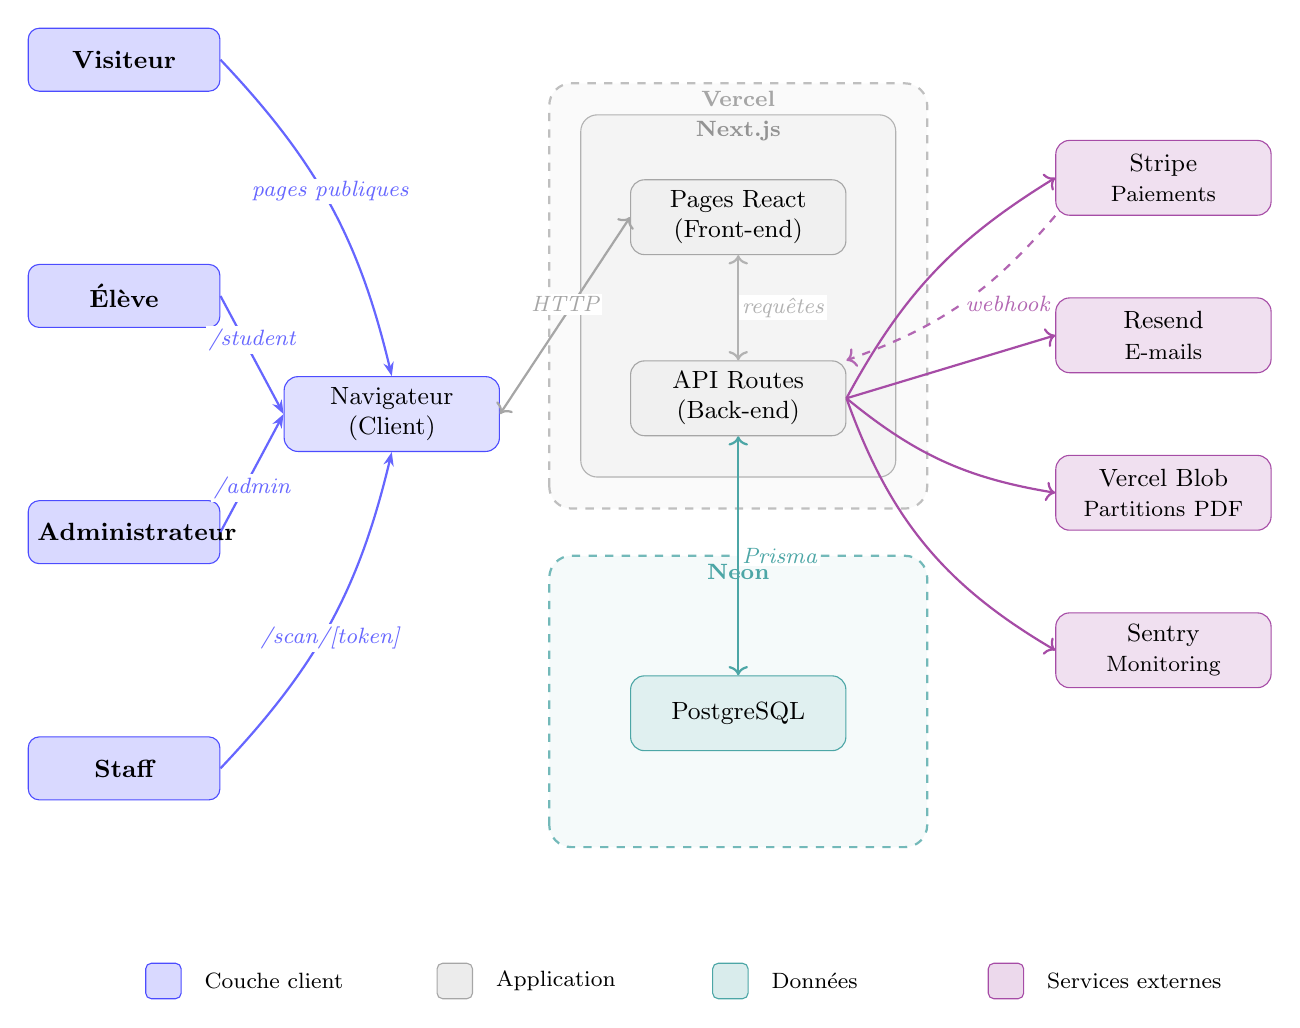
\begin{tikzpicture}[
  every node/.style={font=\small},
  block/.style={rectangle, rounded corners=5pt, draw=#1!70, fill=#1!12,
                text width=2.5cm, align=center, minimum height=0.95cm},
  actor/.style={rectangle, rounded corners=4pt, draw=#1!70, fill=#1!15,
                text width=2.2cm, align=center, minimum height=0.8cm, font=\small\bfseries},
  arr/.style={-{Stealth[length=5pt]}, thick, #1},
  lbl/.style={font=\footnotesize\itshape, fill=white, inner sep=1pt},
  legsq/.style={rectangle, rounded corners=2pt, draw=#1!70, fill=#1!15,
                minimum width=0.45cm, minimum height=0.45cm, inner sep=0pt},
]

% ── Boîtes d'hébergement ─────────────────────────────────────────────

% Vercel (boîte extérieure — gris, même catégorie que l'application)
\draw[rounded corners=8pt, draw=gray!50, fill=gray!4, dashed, thick]
  (5.2, -1.2) rectangle (10.0, 4.2);
\node[font=\footnotesize\bfseries, gray!70] at (7.6, 4.0) {Vercel};

% Next.js (boîte intérieure — gris solide)
\draw[rounded corners=6pt, draw=gray!60, fill=gray!9]
  (5.6, -0.8) rectangle (9.6, 3.8);
\node[font=\footnotesize\bfseries, gray!85] at (7.6, 3.6) {Next.js};

% Neon (boîte autour de PostgreSQL — vert)
\draw[rounded corners=8pt, draw=teal!55, fill=teal!4, dashed, thick]
  (5.2, -5.5) rectangle (10.0, -1.8);
\node[font=\footnotesize\bfseries, teal!70] at (7.6, -2.0) {Neon};

% ── Acteurs (bleu — couche client) ───────────────────────────────────
\node[actor=blue] (vis) at (-0.2,  4.5) {Visiteur};
\node[actor=blue] (etu) at (-0.2,  1.5) {Élève};
\node[actor=blue] (adm) at (-0.2, -1.5) {Administrateur};
\node[actor=blue] (sta) at (-0.2, -4.5) {Staff};

% ── Navigateur (bleu — couche client) ────────────────────────────────
\node[block=blue] (browser) at (3.2, 0.0) {Navigateur\\(Client)};

% ── Composants Next.js (gris — application) ──────────────────────────
\node[block=gray] (frontend) at (7.6,  2.5) {Pages React\\(Front-end)};
\node[block=gray] (api)      at (7.6,  0.2) {API Routes\\(Back-end)};

% ── Base de données (vert — données) ─────────────────────────────────
\node[block=teal] (db) at (7.6, -3.8) {PostgreSQL};

% ── Services externes (violet) ───────────────────────────────────────
\node[block=violet] (stripe) at (13.0,  3.0) {Stripe\\{\footnotesize Paiements}};
\node[block=violet] (resend) at (13.0,  1.0) {Resend\\{\footnotesize E-mails}};
\node[block=violet] (blob)   at (13.0, -1.0) {Vercel Blob\\{\footnotesize Partitions PDF}};
\node[block=violet] (sentry) at (13.0, -3.0) {Sentry\\{\footnotesize Monitoring}};

% ── Flèches acteurs → navigateur (bleu) ──────────────────────────────
\draw[arr=blue!60] (vis.east) to[bend left=15]
  node[lbl, midway, above] {\footnotesize pages publiques} (browser.north);
\draw[arr=blue!60] (etu.east) --
  node[lbl, midway, above] {\footnotesize /student} (browser.west);
\draw[arr=blue!60] (adm.east) --
  node[lbl, midway, below] {\footnotesize /admin} (browser.west);
\draw[arr=blue!60] (sta.east) to[bend right=15]
  node[lbl, midway, below] {\footnotesize /scan/[token]} (browser.south);

% ── Navigateur → Front-end (HTTP) ────────────────────────────────────
\draw[arr=gray!70, <->] (browser.east) -- (frontend.west)
  node[lbl, midway, above] {HTTP};

% ── Front-end ↔ API Routes ───────────────────────────────────────────
\draw[arr=gray!60, <->] (frontend.south) -- (api.north)
  node[lbl, midway, right] {requêtes};

% ── API Routes ↔ PostgreSQL via Prisma ───────────────────────────────
\draw[arr=teal!70, <->] (api.south) -- (db.north)
  node[lbl, midway, right] {Prisma};

% ── API Routes → Services externes ───────────────────────────────────
\draw[arr=violet!70, ->] (api.east) to[bend left=15] (stripe.west);
\draw[arr=violet!60, ->, dashed] (stripe.south west) to[bend left=15]
  node[lbl, midway, right] {\footnotesize webhook} (api.north east);
\draw[arr=violet!70, ->] (api.east) -- (resend.west);
\draw[arr=violet!70, ->] (api.east) to[bend right=15] (blob.west);
\draw[arr=violet!70, ->] (api.east) to[bend right=20] (sentry.west);

% ── Légende ──────────────────────────────────────────────────────────
\node[legsq=blue]   at (0.3,  -7.2) {};
\node[font=\footnotesize, anchor=west] at (0.7, -7.2) {Couche client};
\node[legsq=gray]   at (4.0,  -7.2) {};
\node[font=\footnotesize, anchor=west] at (4.4, -7.2) {Application};
\node[legsq=teal]   at (7.5,  -7.2) {};
\node[font=\footnotesize, anchor=west] at (7.9, -7.2) {Données};
\node[legsq=violet] at (11.0, -7.2) {};
\node[font=\footnotesize, anchor=west] at (11.4, -7.2) {Services externes};

\end{tikzpicture}
}%
\caption{Schéma de l'architecture applicative}
\label{fig:architecture}
\end{figure}

\subsection{Structure du projet}

Le projet suit la convention de structure imposée par \textit{Next.js} 
avec l'App Router. Les principaux dossiers sont organisés comme suit :

\begin{itemize}
    \item \texttt{app/} : contient l'ensemble des pages et des 
    API Routes de l'application, organisées selon la convention 
    de routage de Next.js
    \begin{itemize}
        \item \texttt{app/admin/} : pages réservées à l'interface 
        d'administration, incluant la gestion des cours, des 
        inscriptions, des événements, des séances et des présences
        \item \texttt{app/api/} : API Routes exposant les endpoints 
        HTTP, notamment la connexion, le webhook Stripe et la 
        validation des billets
        \item \texttt{app/student/} : espace personnel des élèves
        \item \texttt{app/event/} : pages publiques des événements 
        et flux de paiement via Stripe
        \item \texttt{app/inscription/} : formulaire d'inscription 
        et page de confirmation
        \item \texttt{app/scan/[token]/} : page de scan des QR 
        codes accessible via lien temporaire
        \item \texttt{app/activation/} : page d'activation du 
        compte via lien d'invitation
    \end{itemize}
    \item \texttt{lib/} : fonctions utilitaires partagées entre 
    les différentes parties de l'application
    \begin{itemize}
        \item \texttt{session.ts} : gestion des sessions utilisateur
        \item \texttt{email.ts} : fonctions d'envoi d'e-mails via Resend
        \item \texttt{ticket-pdf.ts} : génération des billets au 
        format PDF avec QR code
        \item \texttt{prisma.ts} : initialisation et export du 
        client Prisma
    \end{itemize}
    \item \texttt{prisma/} : schéma de la base de données et 
    historique des migrations générées via \texttt{prisma migrate dev}
    \item \texttt{test/} : tests unitaires organisés en miroir 
    de la structure du projet
    \item \texttt{public/} : fichiers statiques tels que les 
    images des cours et les icônes
    \item \texttt{scripts/} : scripts utilitaires, notamment 
    le script de seed pour initialiser la base de données
\end{itemize}

L'ensemble du projet est développé en \textit{TypeScript}. 
Deux extensions sont utilisées selon la nature du fichier : 
\texttt{.tsx} pour les fichiers contenant des composants 
\textit{React} avec du JSX, tels que les pages et les 
composants de l'interface, et \texttt{.ts} pour les fichiers 
de logique pure sans interface, tels que les utilitaires 
du dossier \texttt{lib/} et les API Routes.

\subsection{API Routes}

Dans le cadre de ce projet, les API Routes de \textit{Next.js} ont 
été utilisées pour implémenter la logique serveur de l'application. 
Contrairement à l'utilisation d'une API externe, ces routes sont 
développées directement au sein du projet sous forme de fichiers 
\texttt{route.ts}, organisés dans le dossier \texttt{app/api/}.

Chaque route expose un ou plusieurs points d'entrée HTTP (GET, POST, 
PUT, DELETE) permettant au front-end de communiquer avec le back-end 
de manière structurée. C'est également depuis ces routes que les 
services externes sont consommés, notamment :

\begin{itemize}
    \item \textbf{Prisma} : utilisé pour interagir avec la base 
    de données PostgreSQL, notamment pour lire ou écrire des 
    données relatives aux élèves, aux cours, aux inscriptions 
    et aux paiements
    \item \textbf{Stripe} : appelé pour créer des sessions de 
    paiement et recevoir les webhooks de confirmation de transaction
    \item \textbf{Resend} : utilisé pour envoyer les e-mails 
    transactionnels tels que les confirmations d'inscription 
    et les billets d'événements
    \item \textbf{Vercel Blob} : utilisé pour uploader et 
    récupérer les partitions PDF mises à disposition des élèves
\end{itemize}

Cette approche centralise toute la logique métier côté serveur, 
garantissant que les données sensibles et les clés d'API des 
services externes ne sont jamais exposées côté client.

\subsection{Flux de paiement Stripe}

L'intégration de \textit{Stripe} repose sur un flux en plusieurs 
étapes, impliquant une communication entre le navigateur du visiteur, 
les API Routes de l'application et les serveurs Stripe. La figure 
\ref{fig:flux-stripe} illustre ce flux de manière détaillée.


\begin{figure}[H]
\centering
\resizebox{\linewidth}{!}{%
\begin{tikzpicture}[
  every node/.style={font=\small},
  actor/.style={rectangle, rounded corners=3pt, draw=#1!70, fill=#1!15,
                text width=2.6cm, align=center, minimum height=0.85cm, font=\small\bfseries},
  msg/.style={font=\footnotesize, fill=white, inner sep=1pt},
  arr/.style={-{Stealth[length=5pt]}, thick, #1},
  selfbox/.style={rectangle, rounded corners=2pt, draw=gray!50, fill=gray!8,
                  text width=3.2cm, align=center, font=\footnotesize, minimum height=0.7cm},
]

\def\xV{0} \def\xA{3.8} \def\xS{7.6} \def\xR{11.4}

% Acteurs
\node[actor=blue]   at (\xV,0) {Visiteur};
\node[actor=gray]   at (\xA,0) {Application\\Next.js};
\node[actor=purple] at (\xS,0) {Stripe};
\node[actor=teal]   at (\xR,0) {Resend};

% Lifelines
\foreach \x in {\xV,\xA,\xS,\xR}
  \draw[gray!25, dashed, line width=0.6pt] (\x,-0.45) -- (\x,-9.2);

% 1. Visiteur → Application
\draw[arr=blue!70] (\xV,-1.1) -- (\xA,-1.1)
  node[msg, midway, above] {\textbf{1.} Clic «~Réserver~»};

% 2. Application → Stripe
\draw[arr=gray!70] (\xA,-2.0) -- (\xS,-2.0)
  node[msg, midway, above] {\textbf{2.} Créer session checkout};

% 3. Stripe → Application
\draw[arr=purple!70] (\xS,-2.9) -- (\xA,-2.9)
  node[msg, midway, above] {\textbf{3.} Retourne sessionId};

% 4. Application → Visiteur
\draw[arr=gray!70] (\xA,-3.8) -- (\xV,-3.8)
  node[msg, midway, above] {\textbf{4.} Redirection Checkout};

% 5. Visiteur → Stripe
\draw[arr=blue!70] (\xV,-4.7) -- (\xS,-4.7)
  node[msg, midway, above] {\textbf{5.} Saisie et validation paiement};

% 6. Stripe → Application (webhook)
\draw[arr=purple!70] (\xS,-5.6) -- (\xA,-5.6)
  node[msg, midway, above] {\textbf{6.} Webhook confirmé};

% 7. Application (self — génération PDF)
\node[selfbox] at (\xA,-6.6) {\textbf{7.} Génération billet PDF + QR code};

% 8. Application → Resend
\draw[arr=gray!70] (\xA,-7.5) -- (\xR,-7.5)
  node[msg, midway, above] {\textbf{8.} Envoi email + billet};

% 9. Resend → Visiteur
\draw[arr=teal!70] (\xR,-8.4) -- (\xV,-8.4)
  node[msg, midway, above] {\textbf{9.} Réception billet PDF};

\end{tikzpicture}
}%
\caption{Flux de paiement Stripe — de l'achat à la réception du billet}
\label{fig:flux-stripe}
\end{figure}


\subsection{Pipeline CI/CD}

Afin de garantir la qualité du code et d'automatiser le déploiement, 
un pipeline d'intégration et de déploiement continus a été mis en place, 
reposant sur deux outils complémentaires : \textit{GitHub Actions} et 
\textit{Vercel}.

À chaque \textit{push} vers le dépôt GitHub, GitHub Actions déclenche 
automatiquement une série de vérifications, notamment l'analyse statique 
du code et l'exécution des tests unitaires. Si l'une de ces vérifications 
échoue, le pipeline est interrompu et le déploiement est bloqué, empêchant 
ainsi la mise en production d'un code défaillant.

Si toutes les vérifications sont passées avec succès, \textit{Vercel} 
prend le relais et déploie automatiquement la nouvelle version de 
l'application. Cette intégration permet de maintenir en permanence une 
version stable et fonctionnelle en production, sans intervention manuelle.

Le flux complet peut être résumé comme suit :

\begin{enumerate}
    \item Le développeur pousse le code sur GitHub
    \item GitHub Actions exécute les vérifications (lint, tests)
    \item En cas d'échec, le pipeline est interrompu et le développeur 
    est notifié
    \item En cas de succès, Vercel déploie automatiquement 
    la nouvelle version de l'application en production.
\end{enumerate}

La figure \ref{fig:cicd} illustre ce pipeline de manière schématique.

\begin{figure}[H]
\centering
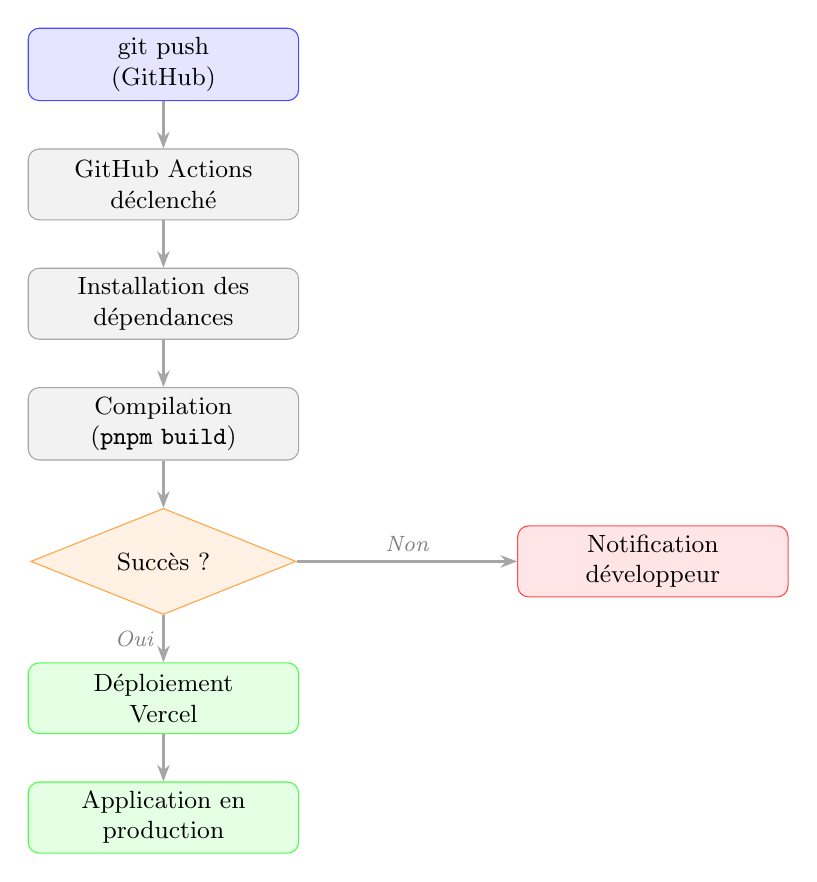
\begin{tikzpicture}[
  node distance=0.6cm and 1.2cm,
  box/.style={rectangle, rounded corners=4pt, draw=#1!70, fill=#1!10,
              text width=3.2cm, align=center, minimum height=0.9cm, font=\small},
  decision/.style={diamond, draw=orange!70, fill=orange!10,
                   text width=2cm, align=center, font=\small, aspect=2.5},
  arrow/.style={-{Stealth[length=6pt]}, thick, gray!70},
  label/.style={font=\footnotesize\itshape, gray}
]

\node[box=blue]   (push)    {git push\\(GitHub)};
\node[box=gray, below=of push]  (actions) {GitHub Actions\\déclenché};
\node[box=gray, below=of actions] (install) {Installation des\\dépendances};
\node[box=gray, below=of install] (build)   {Compilation\\(\texttt{pnpm build})};
\node[decision,  below=of build]  (check)   {Succès ?};
\node[box=green, below=of check]  (deploy)  {Déploiement\\Vercel};
\node[box=green, below=of deploy] (prod)    {Application en\\production};
\node[box=red,   right=2.8cm of check] (notif) {Notification\\développeur};

\draw[arrow] (push)    -- (actions);
\draw[arrow] (actions) -- (install);
\draw[arrow] (install) -- (build);
\draw[arrow] (build)   -- (check);
\draw[arrow] (check)   -- node[label, left]{Oui} (deploy);
\draw[arrow] (deploy)  -- (prod);
\draw[arrow] (check)   -- node[label, above]{Non} (notif);

\end{tikzpicture}
\caption{Schéma du pipeline CI/CD}
\label{fig:cicd}
\end{figure}

\subsection{Variables d'environnement}

Le bon fonctionnement de l'application repose sur la configuration 
de plusieurs variables d'environnement, regroupant les clés d'accès 
aux services externes. Ces variables constituent des informations 
sensibles permettant d'établir une connexion sécurisée avec chaque 
service tiers utilisé par l'application.

Afin de ne jamais exposer ces informations dans le code source, 
elles sont stockées dans un fichier \texttt{.env} en environnement 
local, exclu du dépôt GitHub via le fichier \texttt{.gitignore}. 
Un fichier \texttt{.env.example} a également été fourni dans le 
dépôt, reprenant la structure des variables nécessaires sans 
inclure les valeurs réelles, permettant ainsi à tout développeur 
de configurer son environnement facilement.

En production, ces variables sont configurées directement depuis 
le tableau de bord \textit{Vercel} et injectées automatiquement 
lors du déploiement, sans jamais apparaître dans le code source.

Les principales variables utilisées sont les suivantes :

\begin{itemize}
    \item \textbf{Base de données} :
    \begin{itemize}
        \item \texttt{DATABASE\_URL} : URL de connexion principale 
        à la base de données PostgreSQL hébergée sur Neon, utilisée 
        par Prisma pour les requêtes
        \item \texttt{DIRECT\_URL} : URL de connexion directe à 
        la base de données, utilisée par Prisma lors des migrations
    \end{itemize}

    \item \textbf{Paiements} :
    \begin{itemize}
        \item \texttt{STRIPE\_SECRET\_KEY} : clé secrète Stripe 
        pour les appels API côté serveur
        \item \texttt{STRIPE\_WEBHOOK\_SECRET} : clé de validation 
        des webhooks Stripe, permettant de vérifier que les 
        notifications reçues proviennent bien de Stripe
    \end{itemize}

    \item \textbf{E-mails} :
    \begin{itemize}
        \item \texttt{RESEND\_API\_KEY} : clé d'accès au service 
        d'envoi d'e-mails Resend
    \end{itemize}

    \item \textbf{Application} :
    \begin{itemize}
        \item \texttt{APP\_URL} : URL publique de l'application, 
        utilisée notamment pour générer les liens d'activation 
        de compte et de réinitialisation de mot de passe
        \item \texttt{SESSION\_SECRET} : clé secrète utilisée 
        pour signer et vérifier les cookies de session, garantissant 
        leur intégrité et empêchant toute falsification
    \end{itemize}
\end{itemize}

\section{Méthodologie de travail}

\subsection{Approche incrémentale}

Le développement a suivi une approche incrémentale, découpée 
en plusieurs itérations successives. Une première version 
fonctionnelle (MVP) a été livrée fin mars 2026, couvrant 
les fonctionnalités essentielles : authentification, gestion 
des étudiants et des cours, ainsi que la billetterie en ligne 
avec paiement via Stripe.

Cette version a été présentée au client lors d'une réunion de 
validation, permettant d'identifier les ajustements nécessaires 
et de prioriser les développements suivants. Chaque itération 
ultérieure a fait l'objet d'une présentation au client, 
garantissant une adéquation continue entre les développements 
réalisés et ses attentes.

Cette organisation flexible a également permis de réagir aux 
aléas du projet, notamment les difficultés de connexion à la 
base de données en environnement local ou les problèmes de 
configuration du pipeline CI/CD, sans remettre en cause 
l'avancement global.

\subsection{Gestion de la relation client}

Tout au long du projet, une communication régulière a été maintenue avec 
le client afin de s'assurer que les développements réalisés correspondaient 
bien à ses attentes. Des réunions hebdomadaires ont été organisées afin de 
faire le point sur l'avancement du projet, de valider les fonctionnalités 
implémentées et d'identifier de nouveaux besoins.

En complément, des échanges ont également été menés avec des élèves de 
l'école, dans le but de recueillir leurs attentes concernant l'espace 
personnel qui leur serait destiné. Ces retours ont permis d'orienter 
certains choix fonctionnels afin de proposer une interface adaptée à leurs 
besoins et facilitant leur suivi au sein des cours.

\subsection{Gestion des tâches}

Afin d'organiser le travail de manière structurée, l'outil \textit{GitHub 
Projects} a été utilisé pour planifier et suivre l'avancement des tâches 
tout au long du développement.

Les fonctionnalités à implémenter ont été priorisées selon la méthode 
\textit{MoSCoW}, qui distingue quatre niveaux de priorité :

\begin{itemize}
    \item \textbf{Must have} : fonctionnalités indispensables au bon 
    fonctionnement de l'application, telles que la gestion des inscriptions 
    et le suivi des présences
    \item \textbf{Should have} : fonctionnalités importantes mais non 
    bloquantes, telles que la gestion des paiements en ligne
    \item \textbf{Could have} : fonctionnalités souhaitables si le temps 
    le permettait, telles que la création d'événements avec billetterie
    \item \textbf{Won't have} : fonctionnalités explicitement écartées 
    du périmètre du projet, comme une application mobile
\end{itemize}

Chaque tâche a été rédigée sous la forme d'un \textit{user story}, 
suivant le format : \textit{"En tant que [rôle], je souhaite [action] 
afin de [bénéfice]"}. Cette approche permet de centrer chaque tâche 
sur le besoin concret de l'utilisateur plutôt que sur un aspect 
purement technique. À titre d'exemple :

\begin{itemize}
    \item \textit{"En tant qu'administrateur, je souhaite enregistrer 
    la présence des élèves afin de suivre leur assiduité"}
    \item \textit{"En tant qu'élève, je souhaite consulter mon statut 
    de paiement afin de savoir si je suis en ordre"}
    \item \textit{"En tant que visiteur, je souhaite acheter un billet 
    en ligne afin d'assister à un événement de l'école"}
\end{itemize}
Cette approche a permis de maintenir un développement centré sur les 
besoins prioritaires du client, tout en gardant une vision claire des 
tâches restantes et de leur ordre d'implémentation.

\subsection{Déroulement du développement}

Le développement de l'application a suivi une progression logique,
en commençant par la mise en place de l'infrastructure technique de
base avant d'intégrer progressivement les fonctionnalités métier et
les services externes. Le projet s'est déroulé sur une période de
environ trois mois, de février à mai 2026.

\begin{table}[H]
\centering
\renewcommand{\arraystretch}{1.4}
\begin{tabular}{>{\bfseries}p{3.5cm} p{10cm}}
\toprule
\textbf{Période} & \textbf{Travaux réalisés} \\
\midrule
22 février 2026 & 
Initialisation du projet : création du dépôt GitHub, 
configuration de Next.js et mise en place de l'environnement 
de développement. \\

7 mars 2026 & 
Infrastructure de base : configuration de Prisma avec PostgreSQL 
sur Neon, authentification avec gestion des rôles et des sessions, 
gestion des étudiants et des cours. \\

7--8 mars 2026 & 
Fonctionnalités métier principales : gestion des inscriptions 
avec règles métier, portail étudiant et dashboard administrateur. \\

8 mars 2026 & 
Gestion des événements : création depuis le dashboard, 
page publique pour les visiteurs. \\

14--15 mars 2026 & 
Intégration de Stripe : flux de checkout, webhook de 
confirmation de paiement. \\

22--29 mars 2026 & 
Billetterie complète : envoi du billet PDF avec QR code, 
validation des billets à l'entrée. \textbf{— MVP livré} \\

13--16 avril 2026 & 
CI/CD et qualité : GitHub Actions, Vitest, premiers tests 
unitaires, correction du problème de prefetch. \\

18--23 avril 2026 & 
Planification des séances et gestion des présences par séance. \\

26 avril 2026 & 
Gestion des inscriptions avancée : formulaire avec gestion 
parentale, activation de compte via lien d'invitation. \\

2--9 mai 2026 & 
Contrôle d'accès événements (scan QR temporaire), ressources 
pédagogiques, suivi du solde, intégration Sentry, 
réinitialisation de mot de passe. \\

17--25 mai 2026 & 
Déclaration de paiement par virement, internationalisation 
FR/TR, page des tarifs publique. \\

28--29 mai 2026 & 
Sécurisation (iron-session, ScanToken, ressources PDF privées), 
tableau de bord admin, calendrier étudiant, système de 
facturation par mode de paiement, gestion des tarifs 
avec préavis. \\
\bottomrule
\end{tabular}
\caption{Chronologie du développement}
\label{tab:timeline}
\end{table}

Il est important de noter que le schéma de base de données n'a pas
été figé dès le début du projet. Au fur et à mesure du développement
des fonctionnalités, de nouvelles tables et relations ont été ajoutées
au schéma \textit{Prisma} afin de répondre aux besoins émergents.
Cette évolution progressive du schéma illustre la nature itérative
du développement, où les besoins se précisent au fil de l'avancement
du projet.

Chaque migration du schéma a été gérée via la commande
\texttt{prisma migrate dev}, qui permet de générer et d'appliquer
automatiquement les modifications de la base de données tout en
conservant un historique des changements effectués.

\section{Difficultés rencontrées}

\subsection{Déconnexion involontaire dans l'espace administrateur}

Une première difficulté a été rencontrée concernant la navigation dans 
l'espace administrateur. Après connexion, chaque tentative d'accès à un 
autre onglet du portail admin entraînait une redirection systématique vers 
la page de connexion.

Dans un premier temps, un problème lié au cookie de session a été suspecté. 
Une vérification et un ajustement de sa configuration ont donc été effectués, 
notamment en remplaçant \texttt{secure: true} par une valeur conditionnelle 
adaptée à l'environnement d'exécution. Cette modification constituait une 
bonne pratique, mais elle n'était pas la cause principale du problème.

Après analyse, il s'est avéré que l'erreur provenait du mécanisme de 
\textit{prefetch} de Next.js, qui permet de précharger certaines pages à 
l'avance pour améliorer la navigation. Or, le portail administrateur 
contenait un lien de déconnexion défini comme suit :

\begin{verbatim}
<Link href="/logout">Se déconnecter</Link>
\end{verbatim}

Next.js préchargeait automatiquement cette route, ce qui déclenchait une 
requête \texttt{GET /logout} et supprimait involontairement la session 
utilisateur. En conséquence, l'administrateur était automatiquement 
déconnecté dès la navigation dans l'espace admin.

Le problème a été résolu en désactivant le préchargement de ce lien grâce 
à l'attribut \texttt{prefetch=\{false\}}, ce qui a permis de rétablir un 
comportement normal de la session.

\subsection{Erreurs de connexion à la base de données en environnement local}

Une seconde difficulté technique a été rencontrée lors des tests en 
environnement local. Des erreurs de type \textit{timeout} (\texttt{ETIMEDOUT}) 
survenaient lors des requêtes vers la base de données, notamment lors de 
la connexion ou de la consultation des événements.

Afin d'identifier l'origine du problème, plusieurs vérifications ont été 
effectuées : la configuration des variables d'environnement, les URLs de 
connexion à la base de données ainsi que le schéma Prisma. Malgré ces 
vérifications, le problème persistait.

Il s'est finalement avéré que l'origine du dysfonctionnement n'était pas 
liée au code de l'application, mais à l'environnement réseau utilisé. Le 
réseau Wi-Fi public bloquait certaines connexions sortantes vers la base 
de données hébergée sur Neon, entraînant des délais d'attente. Le problème 
a été résolu en utilisant une connexion mobile (4G).

Cette situation met en évidence l'importance de prendre en compte 
l'environnement réseau lors du développement d'une application reposant 
sur des services cloud externes.

\subsection{Définition du périmètre fonctionnel}

Une troisième difficulté, d'ordre davantage fonctionnel que technique, 
a été rencontrée lors de la définition des fonctionnalités à développer. 
Le client s'étant rapidement déclaré satisfait des fonctionnalités de base 
ainsi que de la vitrine de l'application, il a été nécessaire d'identifier 
de manière autonome des fonctionnalités supplémentaires susceptibles 
d'apporter une réelle valeur ajoutée au projet.

Après consultation du promoteur et des élèves de l'école, plusieurs 
pistes ont été explorées afin de proposer des fonctionnalités facilitant 
l'organisation des cours et améliorant l'expérience des utilisateurs. 
Cette démarche a conduit à l'ajout de fonctionnalités telles que la 
gestion des événements avec billetterie en ligne, la génération automatique 
de billets PDF avec QR code, ainsi que la mise en place d'un système de 
contrôle d'accès via lien temporaire.

Cette expérience a mis en évidence l'importance de ne pas se limiter aux 
attentes initiales du client, mais de faire preuve d'initiative afin de 
proposer une solution complète et évolutive.

\subsection{Crashs du compilateur Turbopack en développement}
Un comportement inattendu a été observé en environnement de développement :
des crashs fatals survenaient régulièrement au niveau du compilateur
Turbopack, intégré par défaut dans Next.js 16. Ces erreurs n'affectaient
pas la production, mais perturbaient le rechargement à chaud
(\textit{hot reload}), rendant les tests locaux peu fiables.

Afin d'en identifier la cause, les fichiers de panique générés
automatiquement par Turbopack ont été analysés. Ces fichiers, situés dans
\texttt{/tmp/next-panic-*.log}, ont révélé que le compilateur tentait de
construire la route \texttt{/admin/scan/page}, pourtant supprimée lors
d'un commit précédent. L'entrée correspondante persistait dans le cache
de compilation \texttt{.next}, ce qui provoquait une erreur interne à
chaque tentative de rechargement.

Le problème a été résolu en supprimant ce cache via la commande
\texttt{rm -rf .next}, forçant ainsi Turbopack à reconstruire l'intégralité
de l'arbre des routes depuis zéro.

Cette situation illustre l'importance de vider le cache de compilation
après la suppression de routes dans un projet Next.js, afin d'éviter
des incohérences entre le système de fichiers et l'état interne du
compilateur.

\section{Sécurité}

La sécurité de l'application a été prise en compte dès la conception, 
notamment en ce qui concerne la gestion des accès et la protection des 
données sensibles des utilisateurs.

\subsection{Gestion des rôles et des accès}

L'application distingue quatre types d'utilisateurs, chacun disposant 
d'un niveau d'accès bien défini :

\begin{itemize}
    \item \textbf{Visiteur} : accès uniquement aux pages publiques 
    de l'application, telles que la vitrine, la liste des cours 
    disponibles et les événements à venir
    \item \textbf{Élève} : accès à son espace personnel après 
    authentification, lui permettant de consulter son historique 
    de présences et son statut de paiement
    \item \textbf{Administrateur} : accès complet à l'interface 
    d'administration, permettant de gérer les élèves, les cours, 
    les inscriptions, les présences et les événements
    \item \textbf{Staff} : accès restreint à la page de scan 
    via un lien temporaire généré par l'administrateur, permettant 
    le contrôle des billets lors des événements sans disposer 
    d'un accès complet à l'interface d'administration
\end{itemize}

\subsection{Protection des routes}

Les routes de l'application sont protégées côté serveur via un 
mécanisme de vérification de session. À chaque requête vers une 
page ou une API Route protégée, le système vérifie si l'utilisateur 
est authentifié et si son rôle lui autorise l'accès à la ressource 
demandée. Dans le cas contraire, il est redirigé vers la page de 
connexion.

\subsection{Accès temporaire pour le contrôle des billets}

Pour la gestion des événements, un mécanisme d'accès temporaire a 
été mis en place afin de permettre à un membre du staff de scanner 
les QR codes à l'entrée, sans disposer d'un accès complet à 
l'interface d'administration. L'administrateur génère un lien 
temporaire donnant accès uniquement à la page de scan. Ce lien 
expire après une durée définie, limitant ainsi les risques en cas 
d'utilisation non autorisée.

\subsection{Sécurisation de l'endpoint de validation}

Dans l'implémentation initiale, l'endpoint de validation des 
billets était entièrement public. Toute personne connaissant 
l'identifiant unique d'un billet pouvait appeler directement 
la route de validation et rendre le QR code invalide, sans 
être authentifiée ni faire partie du staff.

Cette vulnérabilité a été corrigée en intégrant la vérification 
du \textit{ScanToken} dans l'endpoint de validation. Désormais, 
toute requête de validation doit obligatoirement inclure un 
token temporaire valide, généré par l'administrateur et lié à 
un événement précis. Un utilisateur extérieur ne disposant pas 
de ce token se voit systématiquement refuser l'accès, garantissant 
que seuls les membres du staff autorisés peuvent valider des billets.

\subsection{Hachage des mots de passe}

Les mots de passe des utilisateurs ne sont jamais stockés en clair 
dans la base de données. Ils sont hachés et salés avant d'être 
enregistrés, ce qui garantit leur protection dans deux cas de figure :

\begin{itemize}
    \item \textbf{En cas de compromission de la base de données} : 
    même si un attaquant accède aux données, il ne peut pas 
    retrouver les mots de passe originaux à partir des hachés
    \item \textbf{Contre les attaques par table arc-en-ciel} 
    (\textit{rainbow table}) : le sel ajouté au mot de passe avant 
    le hachage rend ces attaques inefficaces, car deux mots de passe 
    identiques produiront des hachés différents
\end{itemize}

\subsection{Politique de mot de passe}
Lors de l'activation du compte via le lien d'invitation, l'utilisateur 
est invité à définir son mot de passe. Une politique de complexité a été 
mise en place afin de garantir un niveau de sécurité minimal. Le mot de 
passe doit respecter les critères suivants :
\begin{itemize}
    \item Au moins 8 caractères
    \item Au moins une lettre majuscule
    \item Au moins un chiffre
    \item Au moins un caractère spécial
\end{itemize}
Cette validation est effectuée côté serveur, dans la Server Action 
chargée de l'activation du compte, avant tout traitement de la requête. 
Elle vient compléter le hachage des mots de passe avec \textit{argon2}, 
garantissant ainsi que les mots de passe stockés sont à la fois 
robustes et protégés.

\subsection{Sécurité des paiements}

La gestion des paiements est entièrement déléguée à \textit{Stripe}, 
ce qui signifie qu'aucune donnée bancaire sensible ne transite par 
les serveurs de l'application. Les informations de carte sont saisies 
directement dans une interface sécurisée fournie par Stripe, conforme 
à la norme \textit{PCI DSS} qui encadre la sécurité des transactions 
par carte bancaire.

\subsection{Conformité RGPD}

Le \textit{RGPD}~\cite{rgpd} (Règlement Général sur la Protection des Données) 
est une réglementation européenne qui encadre la collecte, le 
traitement et le stockage des données personnelles des citoyens 
de l'Union européenne. Dans le cadre de ce projet, plusieurs 
mesures ont été prises afin de respecter ces exigences.

L'application collecte des données personnelles telles que les 
noms, prénoms et adresses e-mail des élèves, ainsi que des 
informations relatives aux paiements. Ces données sont stockées 
dans la base de données hébergée sur \textit{Neon}, dont les 
serveurs sont localisés à Francfort, en Allemagne, au sein de 
l'Union européenne. Cette localisation garantit que les données 
restent soumises au cadre juridique européen.

De plus, les mots de passe des utilisateurs sont hachés et salés 
via \textit{argon2}, limitant ainsi les risques en cas de 
compromission de la base de données. Les paiements sont quant 
à eux entièrement gérés par \textit{Stripe}, certifié 
\textit{PCI DSS}, ce qui évite que des données bancaires 
sensibles transitent par les serveurs de l'application.

La collecte des données personnelles repose sur le consentement 
explicite de l'élève (ou de son représentant légal s'il est mineur), 
recueilli lors de la soumission du formulaire d'inscription. 
Ce consentement porte sur le traitement des données nécessaires 
à la gestion des cours, des présences et des paiements.

Les personnes concernées disposent d'un droit d'accès, de 
rectification et de suppression de leurs données personnelles. 
Ces demandes peuvent être adressées directement à l'administrateur, 
qui est en mesure d'effectuer ces modifications depuis l'interface 
de gestion.

Les données des élèves sont conservées pour la durée de leur 
inscription à l'école. En cas de désinscription, les données 
peuvent être supprimées sur demande, à l'exception des informations 
nécessaires à des obligations légales telles que la conservation 
des données comptables, imposée par la 
législation belge pendant une durée de sept ans~\cite{cde}.

Le consentement est recueilli explicitement via une case à cocher 
obligatoire lors de la soumission du formulaire d'inscription, 
conformément aux exigences du RGPD.

\subsection{Maintenance de la sécurité}

Garantir la sécurité de l'application sur le long terme nécessite 
une vigilance continue après la livraison. Plusieurs actions 
sont à prévoir :

\begin{itemize}
    \item \textbf{Mises à jour des dépendances} : les bibliothèques 
    de sécurité telles qu'\textit{argon2} et \textit{Iron Session} 
    doivent être maintenues à jour afin de bénéficier des correctifs 
    de sécurité publiés par leurs mainteneurs
    \item \textbf{Sauvegardes de la base de données} : des sauvegardes 
    régulières de la base de données hébergée sur \textit{Neon} 
    permettent de prévenir toute perte de données en cas d'incident
    \item \textbf{Rotation de la clé de session} : la variable 
    \texttt{SESSION\_SECRET} devrait être renouvelée périodiquement, 
    ce qui invalide toutes les sessions actives et force une 
    reconnexion des utilisateurs
    \item \textbf{Surveillance active} : \textit{Sentry} détecte 
    automatiquement les erreurs et comportements anormaux, 
    permettant une réaction rapide en cas d'incident de sécurité
\end{itemize}

\section{Limites et perspectives}


\subsection{Maintenance et évolutivité technique}

Comme toute solution web reposant sur des dépendances externes, 
l'application nécessite une maintenance régulière afin de garantir 
sa disponibilité et sa sécurité dans le temps. Les mises à jour de 
\textit{Next.js}, de \textit{Prisma} ou encore les évolutions de 
l'API \textit{Stripe} peuvent introduire des changements incompatibles 
nécessitant des adaptations du code. De même, le compilateur 
\textit{Turbopack}, encore en phase de développement actif, peut 
présenter des instabilités comme cela a été observé durant le projet.

\subsection{Coûts sur le long terme}

L'application repose sur plusieurs services externes dont certains 
sont gratuits dans leurs limites actuelles, mais peuvent engendrer 
des coûts supplémentaires si l'activité du client venait à se 
développer. C'est notamment le cas pour :

\begin{itemize}
    \item \textbf{Vercel} : l'hébergement de l'application est 
    gratuit dans le cadre du plan hobby, mais un passage à un plan 
    payant serait nécessaire en cas d'augmentation significative 
    du trafic ou pour bénéficier de fonctionnalités avancées
    \item \textbf{Neon} : l'hébergement de la base de données 
    PostgreSQL est gratuit jusqu'à un certain volume de données 
    et de connexions simultanées
    \item \textbf{Stripe} : des frais de transaction sont prélevés 
    sur chaque paiement effectué via la plateforme
    \item \textbf{Vercel Blob} : le stockage des partitions PDF 
    est soumis à des limites de capacité dans le plan gratuit
    \item \textbf{Sentry} : la surveillance des erreurs est 
    gratuite jusqu'à 5 000 erreurs par mois. Au-delà de 
    cette limite, un passage à un plan payant serait 
    nécessaire, bien que ce seuil soit largement suffisant 
    pour l'échelle actuelle du projet
\end{itemize}

\subsection{Validation des billets hors ligne}

La validation des billets par scan de QR code nécessite 
une connexion internet, dans la mesure où chaque scan 
déclenche un appel à la base de données afin de vérifier 
la validité du billet et de le marquer comme utilisé. 
En cas de couverture réseau insuffisante lors de 
l'événement, cette fonctionnalité ne peut pas être utilisée.

Afin de pallier cette limitation, chaque billet généré 
affiche les informations nominatives de l'acheteur, 
notamment son nom et son prénom, en complément du QR code. 
Cette approche permet au staff de vérifier visuellement 
l'identité du porteur du billet sans nécessiter de 
connexion réseau, en la confrontant à une pièce d'identité 
si nécessaire.

Il convient toutefois de noter que cette alternative 
visuelle est moins sécurisée que le scan automatique, 
dans la mesure où elle ne détecte pas les utilisations 
multiples d'un même billet. Elle reste cependant 
adaptée au contexte de l'école, dont les événements 
accueillent un public restreint et connu.

\subsection{Gestion mono-administrateur}

L'application a été conçue pour un seul administrateur, 
correspondant au profil actuel du client. Dans le cas où 
l'école viendrait à se développer et à accueillir plusieurs 
professeurs, le système ne permet pas actuellement de gérer 
plusieurs comptes administrateurs disposant chacun de droits 
distincts.

Par exemple, il ne serait pas possible d'attribuer à un 
professeur l'accès uniquement aux cours qu'il dispense, ou 
de restreindre la consultation des données financières à 
certains utilisateurs seulement. Cette limitation reste 
cohérente avec le périmètre défini lors de l'analyse des 
besoins initiaux, mais constitue un frein potentiel si 
l'école venait à engager d'autres enseignants.

\section{Conclusion}

Ce travail de fin d'études a été une expérience enrichissante tant 
sur le plan technique que sur le plan humain et organisationnel.

\subsection*{Bilan technique}

Ce projet a permis d'acquérir de nouvelles compétences dans des 
technologies qui n'avaient pas été abordées durant le parcours 
académique à l'EPHEC. C'est notamment le cas de \textit{Prisma}, 
un ORM permettant d'interagir avec une base de données de manière 
structurée et typée, ainsi que de services cloud modernes tels que 
\textit{Neon}, \textit{Resend}, \textit{Stripe} et 
\textit{Vercel Blob}. La manipulation de ces outils a permis de 
mieux comprendre les interactions entre les différentes couches 
d'une application web moderne et les enjeux liés à l'intégration 
de services externes.

\subsection*{Bilan méthodologique}

Au-delà des compétences techniques, ce projet a mis en évidence 
l'importance de la rigueur et de l'organisation dans le cadre d'un 
développement solo. La mise en place d'une méthodologie structurée, 
notamment à travers l'utilisation de la méthode \textit{MoSCoW} et 
des \textit{user stories}, a permis de maintenir un cap clair tout 
au long du développement et de livrer une solution répondant aux 
besoins réels du client.

Ce projet m'a également permis de prendre conscience de
l'importance de la flexibilité. Au cours du développement,
certains choix initiaux ont dû être revus, qu'il s'agisse
d'éléments d'interface comme le formulaire d'inscription,
ou d'outils techniques comme \textit{Pino}, finalement
remplacé par \textit{Sentry} pour les raisons évoquées
précédemment.

Si c'était à refaire, j'intégrerais la sécurité dès la
conception plutôt que de la traiter comme une correction
à posteriori. Plusieurs vulnérabilités — comme le stockage
des partitions PDF dans un espace public ou l'absence
de chiffrement du cookie de session — n'ont été identifiées
et corrigées qu'après coup, alors qu'elles auraient dû être
anticipées dès l'analyse des besoins. De même, j'écrirais
les tests de manière progressive, en parallèle du
développement de chaque fonctionnalité, plutôt que de les
regrouper en fin de projet.

\subsection*{Bilan humain}

Ce projet a également été formateur sur le plan de la relation 
client. Le client, satisfait des fonctionnalités de base proposées, 
ne formulait pas spontanément de nouvelles demandes. Il a donc été 
nécessaire de faire preuve d'initiative, d'aller à la rencontre du 
client de manière proactive et de lui soumettre des propositions 
concrètes. Cette expérience a mis en évidence que les compétences 
organisationnelles et relationnelles sont tout aussi importantes, 
sinon davantage, que les compétences purement techniques.

\subsection*{Perspectives}

L'application développée constitue une base solide et évolutive 
pour la gestion de l'école de musique. Plusieurs pistes 
d'amélioration ont été identifiées, notamment le développement 
d'une application mobile, l'ajout de notifications push et la 
mise en place d'un tableau de bord statistique. Ces évolutions 
permettraient de renforcer encore davantage la valeur apportée 
au client et de répondre à de futurs besoins.

Ce projet représente une expérience complète de développement 
d'une application web en conditions réelles, depuis l'analyse 
des besoins jusqu'à la mise en production, en passant par les 
choix techniques, la sécurisation et le déploiement continu.


\subsection*{Pérennité de la solution}

Afin de garantir la continuité du service après la livraison, 
plusieurs éléments doivent être pris en compte.

Sur le plan technique, les dépendances du projet devront être 
maintenues à jour régulièrement, notamment \textit{Next.js}, 
\textit{Prisma} et les bibliothèques de sécurité telles 
qu'\textit{argon2} et \textit{Iron Session}. Des mises à jour 
négligées peuvent introduire des failles de sécurité ou des 
incompatibilités avec les services externes.

La base de données hébergée sur \textit{Neon} devrait faire 
l'objet de sauvegardes régulières afin de prévenir toute perte 
de données en cas d'incident. Neon propose une fonctionnalité 
de sauvegarde automatique dans ses plans payants, qu'il serait 
recommandé d'activer si l'application venait à être utilisée 
en production de manière intensive.

Sur le plan financier, les coûts liés aux services externes 
restent maîtrisés dans le cadre actuel, les plans gratuits 
étant suffisants pour une structure d'une quarantaine d'élèves. 
Une réévaluation des plans utilisés serait néanmoins nécessaire 
si l'école venait à se développer significativement.

Enfin, \textit{Sentry} assure une surveillance active de 
l'application après la livraison, permettant de détecter et 
corriger rapidement d'éventuelles erreurs sans nécessiter 
une intervention proactive quotidienne.

\section*{Références bibliographiques}
\begin{thebibliography}{99}

\bibitem{nextjs}
Next.js Documentation. \textit{Next.js by Vercel}.
Consulté en 2026. \url{https://nextjs.org/docs}

\bibitem{prisma}
Prisma Documentation. \textit{Prisma ORM}.
Consulté en 2026. \url{https://www.prisma.io/docs}

\bibitem{postgresql}
PostgreSQL Documentation. \textit{PostgreSQL}.
Consulté en 2026. \url{https://www.postgresql.org/docs}

\bibitem{neon}
Neon Documentation. \textit{Neon Serverless Postgres}.
Consulté en 2026. \url{https://neon.tech/docs}

\bibitem{stripe}
Stripe Documentation. \textit{Stripe Payments}.
Consulté en 2026. \url{https://stripe.com/docs}

\bibitem{resend}
Resend Documentation. \textit{Resend Email API}.
Consulté en 2026. \url{https://resend.com/docs}

\bibitem{vercel}
Vercel Documentation. \textit{Vercel Platform}.
Consulté en 2026. \url{https://vercel.com/docs}

\bibitem{vercelblob}
Vercel Blob Documentation. \textit{Vercel Blob Storage}.
Consulté en 2026. \url{https://vercel.com/docs/storage/vercel-blob}

\bibitem{argon2}
Argon2 — Password Hashing. \textit{OWASP Password Storage Cheat Sheet}.
Consulté en 2026. \url{https://cheatsheetseries.owasp.org/cheatsheets/Password_Storage_Cheat_Sheet.html}

\bibitem{vitest}
Vitest Documentation. \textit{Vitest Unit Testing Framework}.
Consulté en 2026. \url{https://vitest.dev/}

\bibitem{moscow}
Clegg, D. et Barker, R. (1994). \textit{Case Method Fast-Track: A RAD Approach}.
Addison-Wesley. (Méthode MoSCoW)

\bibitem{githubactions}
GitHub Actions Documentation. \textit{GitHub Actions}.
Consulté en 2026. \url{https://docs.github.com/en/actions}

\bibitem{sentry}
Sentry Documentation. \textit{Sentry Error Monitoring}.
Consulté en 2026. \url{https://docs.sentry.io}

\bibitem{cde}
Service Public Fédéral Économie. \textit{Code de droit économique,
article III.86 — Conservation des documents comptables}.
Consulté en 2026. \url{https://economie.fgov.be}

\bibitem{rgpd}
Autorité de Protection des Données (APD). 
\textit{Le Règlement Général sur la Protection des Données}.
Consulté en 2026. \url{https://www.autoriteprotectiondonnees.be}

\end{thebibliography}                                                                                                                                                                                                                                                   

\end{document}
